% ============================================================================
%  Searching Continuous Audio as a Whole Item
%  A Sequence-Individuation Algorithm for Radio, Mixes, and Sets
%
%  Self-contained. Every object is a finite weighted graph or a construction
%  on one. Only standard external literature is cited.
% ============================================================================
\documentclass[11pt,twocolumn,a4paper]{article}

\usepackage[utf8]{inputenc}
\usepackage[T1]{fontenc}
\usepackage{lmodern}
\usepackage[a4paper,margin=2.5cm]{geometry}
\usepackage{amsmath,amssymb,amsthm,mathtools}
\usepackage{bm}
\usepackage{mathrsfs}
\usepackage{booktabs}
\usepackage{array}
\usepackage{enumitem}
\usepackage{microtype}
\usepackage{graphicx}
\usepackage{xcolor}
\usepackage{algorithm}
\usepackage{algpseudocode}
\usepackage[round,sort&compress]{natbib}
\usepackage[colorlinks=true,linkcolor=blue!45!black,
            citecolor=blue!45!black,urlcolor=blue!45!black]{hyperref}
\usepackage{cleveref}

% ---- Theorem environments ----
\newtheoremstyle{thmstyle}{\topsep}{\topsep}{\itshape}{}{\bfseries}{.}{.5em}{}
\theoremstyle{thmstyle}
\newtheorem{theorem}{Theorem}[section]
\newtheorem{lemma}[theorem]{Lemma}
\newtheorem{proposition}[theorem]{Proposition}
\newtheorem{corollary}[theorem]{Corollary}
\theoremstyle{definition}
\newtheorem{definition}[theorem]{Definition}
\newtheorem{axiom}{Axiom}
\newtheorem{problem}{Problem}
\newtheorem{construction}[theorem]{Construction}
\newtheorem{example}[theorem]{Example}
\theoremstyle{remark}
\newtheorem{remark}[theorem]{Remark}
\newtheorem{notation}[theorem]{Notation}

\crefname{axiom}{Axiom}{Axioms}
\Crefname{axiom}{Axiom}{Axioms}
\crefname{problem}{Problem}{Problems}
\Crefname{problem}{Problem}{Problems}

% ---- Operators ----
\DeclareMathOperator*{\argmin}{arg\,min}
\DeclareMathOperator*{\argmax}{arg\,max}

% ---- Shorthand ----
\newcommand{\R}{\mathbb{R}}
\newcommand{\N}{\mathbb{N}}
\newcommand{\Z}{\mathbb{Z}}
\newcommand{\Gph}{\Gamma}
\newcommand{\V}{V}
\newcommand{\E}{E}
\newcommand{\wt}{w}
\newcommand{\med}{\mathsf{m}}
\newcommand{\flo}{\beta}
\newcommand{\cut}{\partial}
\newcommand{\co}{\complement}
\newcommand{\str}{\sigma}
\newcommand{\res}{\rho}
\newcommand{\stream}{\mathcal{S}}
\newcommand{\hand}{h}
\newcommand{\Hand}{\mathcal{H}}
\newcommand{\catl}{\gamma}
\newcommand{\Catl}{\mathcal{C}}
\newcommand{\sig}{\Sigma}
\newcommand{\algn}{a}
\newcommand{\Om}{\Omega}
\newcommand{\dem}{D}
\newcommand{\abs}[1]{\lvert#1\rvert}
\newcommand{\norm}[1]{\lVert#1\rVert}
\newcommand{\eps}{\varepsilon}
\newcommand{\bigOh}{\mathcal{O}}

\title{\textbf{Search Algorithms for Electronic Dance Music Set List Generation: \\[3pt]
A Sequence-Individuation Algorithm for Radio, Mixes, and Sets}}

\author{%
Kundai Farai Sachikonye\\
\small Technical University of Munich\\
\small AIMe Registry for Artificial Intelligence\\
\small \texttt{kundai.sachikonye@wzw.tum.de}}

\date{\today}

\begin{document}
\maketitle

% ============================================================================
\begin{abstract}
\noindent
Audio search is conventionally posed for a single recording: a query clip is
matched against a catalogue of tracks by an acoustic fingerprint. Yet much of
what people listen to is not a track but a \emph{continuous audio item}---a
radio broadcast, a recorded DJ mix, the audio of a party or a live set---that
concatenates dozens of tracks, mostly authored by others, into one artefact.
For such an item the interesting object is not any single constituent but the
\emph{whole}: which stream is this, and what is the sequence it realises? We
give an algorithm that searches a continuous item as a single object. Our
central claim is that the identity of a continuous audio item is not its
\emph{content} (the multiset of tracks it contains, which many items share) but
its \emph{sequence} (the ordered, timed arrangement of those tracks, which is
essentially unique to the item that produced it). We formalise a continuous
item as a walk on a finite weighted \emph{contact graph} whose vertices are
individuated constituents and whose edge weights are the cost of telling one
constituent from another. We prove a \emph{resolution floor}: identifying a
constituent against an open catalogue costs a strictly positive, irreducible
amount, so a constituent is never resolved to a point but only to a bounded
region, and---decisively for efficiency---one should resolve each constituent
only to its \emph{least sufficient identifier}, the cheapest handle (typically
a title or artist name) that suffices to place it, descending to acoustic
features only where a name cannot disambiguate. We prove three structural
properties that make partial, noisy recognition tolerable: \emph{sequence
identity} (two items match iff their constituent sequences align, not their
content sets), \emph{convergence-only admissibility} (a reconstructed sequence
is admissible iff it converges on the target signature, so locally wrong
constituent guesses do not invalidate the match provided the whole sequence
aligns), and \emph{search--match duality} (recognising which known item a query
stream is, and generating a stream in the style of a known item, are the same
computation run in opposite directions). We give the full algorithm---acquisition
of least-sufficient handles, sequence signature construction, and a
gap-tolerant alignment that returns an accounted match together with an explicit
unresolved residual---prove its correctness and $\bigOh(\cdot)$ complexity,
validate every structural result numerically on exact minimum cuts and exact
sequence alignment, and specify an evaluation protocol. The validation makes the
one contingent claim explicit: the whole-item search is cheaper than per-track
fingerprinting only by the \emph{nameable fraction} of the stream (a measured
mean of $3.1\times$, not the worst-case guarantee), because the opening
constituent, having no resolved neighbour, always faces the full pool. The result
is a music search that operates at
the granularity of the listening experience: you search for the \emph{set}, not
for every song in it.
\end{abstract}

\noindent\textbf{Keywords:} audio search; continuous audio; DJ mix
identification; sequence alignment; music information retrieval; contact graph;
minimum cut; least sufficient identifier; resolution floor; gap-tolerant
matching.

\tableofcontents

% ============================================================================
\section{Introduction}
\label{sec:intro}
% ============================================================================

\subsection{The problem of the whole item}

Acoustic search has a canonical shape. A short query recording is reduced to a
compact fingerprint---a sparse set of time--frequency landmarks or a hashed
spectral summary---and matched against an index of per-track fingerprints; a
hit returns the single track the query is a fragment of
\citep{wang2003shazam,haitsma2002fingerprint,cano2005review}. This shape is
extraordinarily effective for its intended use: identify \emph{one} song from a
\emph{fragment} of it.

But a large part of ordinary listening is not a track and is not a fragment. It
is a \emph{continuous audio item}: a radio show, a recorded mix, a festival set,
the ambient audio of a party. Such an item runs from tens of minutes to several
hours and concatenates many tracks---most by other artists---into a single
authored artefact. Confronted with such an item, a listener does not usually
want to identify one embedded song; they want to identify, retrieve, or
characterise the \emph{item itself}: \emph{which} broadcast or set is this, is
this the same set I heard last week, what is its tracklist, and what other
items resemble it.

The single-track paradigm answers this only awkwardly and expensively. To search
a whole item with a track engine one must (i) segment the item into candidate
track regions, (ii) fingerprint each region, (iii) query each fingerprint
against the catalogue, and (iv) somehow reassemble the per-region hits into a
statement about the whole. Steps (i)--(iii) repeat the full acoustic pipeline
dozens of times per item, and step (iv) is left undefined: a bag of recognised
tracks is returned, with no account of \emph{which item} produced them, because
the very thing that distinguishes one item from another---the arrangement---has
been discarded by treating the item as a set of independent lookups.

\subsection{Content is shared; sequence is not}

The defect is not one of engineering effort but of the object being searched
for. Consider two recorded mixes that happen to draw on the same fashionable
selection of twenty tracks. As \emph{content}---as unordered multisets of
constituents---they are identical, and a bag-of-tracks search cannot tell them
apart. Yet they are plainly different items: they order the tracks differently,
transition between them differently, and were assembled by (possibly) different
authors for different occasions. What individuates one continuous item from
another is not \emph{which} constituents appear---those are drawn from a shared,
public pool that many items reuse---but the \emph{order and timing} in which
they appear. Two authors who reliably produced the same ordered sequence would
be indistinguishable and mutually substitutable; that they are not
substitutable is exactly the observation that the sequence, not the content, is
the identity.

This reframes the search task. The object to be individuated is the
\emph{sequence}. The constituents are the alphabet over which sequences are
written, and they are largely shared across items; the item's identity lives in
the string, not in the letters. A correct search for a continuous item is
therefore a search over \emph{sequences of constituents}, and the natural
matching operation is \emph{sequence alignment}
\citep{needleman1970,smith1981}, not set intersection.

\subsection{Just enough to place each letter}

Reframing the object also reframes how hard each constituent must be recognised.
If the identity of the item is its sequence, then a constituent needs to be
resolved only to the point where it can be \emph{placed in the sequence}---told
apart from the other constituents that might occupy that position---and no
further. A constituent embedded in a stream is already heavily constrained by
its neighbours; often a coarse handle (a title, an artist, a coarse acoustic
class) suffices to place it, and computing a full acoustic fingerprint would be
paying to resolve a distinction the sequence has already made.

We make this precise as a \emph{resolution floor} (\Cref{sec:floor}): against an
open, non-exhaustible catalogue, identifying a constituent costs a strictly
positive, irreducible amount, and cannot in principle be driven to zero. Two
consequences follow. First, a constituent is never resolved to an exact point,
only to a bounded region---so search returns regions, and matching is
comparison of regions, not equality of points. Second, and practically
decisive, there is a \emph{least sufficient identifier} for each constituent:
the cheapest handle that already separates it from its plausible alternatives.
Resolving beyond it is wasted work \emph{and}, we argue, a category error---an
attempt at the impossible zero-cost identification. The algorithm therefore
resolves each constituent to its least sufficient identifier and descends to
expensive acoustic features only for constituents a cheap handle cannot place
(an unlabelled or ambiguous constituent---the case where two candidates share a
name but differ acoustically).

\subsection{Robustness, and one engine for two tasks}

Two further structural facts, proved below, make the approach robust and
economical.

\emph{Convergence-only admissibility} (\Cref{sec:matching}). Because matching is
sequence alignment against a target signature, a reconstructed sequence is
admissible as a match iff the \emph{whole} sequence aligns; individual
mis-recognised constituents do not by themselves invalidate the match. A wrong
guess at one position is absorbed as a local substitution or gap, and the match
stands or falls on global convergence. This is exactly the tolerance a
real-world stream demands, where a fraction of constituents are unlabelled or
misheard.

\emph{Search--match duality} (\Cref{sec:duality}). Recognising which known item
a query stream is (analysis) and generating a stream in the manner of a known
item (synthesis) are the same computation over the same object---an alignment on
the contact graph---read in opposite directions. One implementation serves both
``identify this set'' and ``build a set like this one.''

\subsection{Contributions}

\begin{enumerate}[leftmargin=1.4em,itemsep=2pt]
\item \textbf{A problem formulation} (\Cref{sec:model}): continuous audio search
  as the individuation of a \emph{sequence} on a finite weighted contact graph,
  with the identity of an item shown to be its sequence signature and not its
  content set.
\item \textbf{The resolution floor and least sufficient identifier}
  (\Cref{sec:floor}): a proof that constituent identification against an open
  catalogue has a strictly positive irreducible cost, that identity is
  region-valued, and that the cheapest sufficient handle is the correct
  resolution target; a formal cost model follows.
\item \textbf{Sequence identity} (\Cref{sec:signature}): the item signature, and
  a proof that it is invariant under re-encoding of constituent labels while
  content sets are not, so that the signature is the individuating datum.
\item \textbf{A gap-tolerant matching algorithm} (\Cref{sec:matching}) with
  convergence-only admissibility, returning an accounted alignment plus an
  explicit unresolved residual; correctness and complexity are proved.
\item \textbf{Search--match duality} (\Cref{sec:duality}): analysis and synthesis
  as one operation in two directions.
\item \textbf{The full system and its evaluation protocol}
  (\Cref{sec:algorithm,sec:evaluation}): end-to-end pseudocode, complexity, and
  a reproducible measurement design.
\item \textbf{Numerical validation} (\Cref{sec:validation}): a reproducible,
  seeded suite that verifies all $14$ structural results by exact computation on
  constructed and random instances, and quantifies the single contingent claim---%
  the whole-item saving is proportional to the nameable fraction, with a measured
  mean of $3.1\times$ rather than the worst-case bound.
\end{enumerate}

\subsection{Method and scope}

Every object in this paper is a finite weighted graph or a construction on one.
We use minimum cuts, computable exactly by maximum flow
\citep{fordfulkerson1956,menger1927,stoer1997mincut}, as the sole measure of how
costly it is to tell one constituent from another; we use classical sequence
alignment \citep{needleman1970,smith1981} as the sole matching primitive. We
introduce no probability calculus beyond a derived normalisation to $[0,1]$. The
theory is structural: it establishes \emph{that} the identity of a continuous
item is its sequence, \emph{that} constituent resolution is floored and should
stop at the least sufficient handle, and \emph{that} matching is
convergence-only sequence alignment. Concrete acoustic features and a concrete
constituent recogniser are implementation inputs the framework organises but
does not itself supply; where a numerical choice is required we state it as a
parameter and mark it as such.

% ============================================================================
\section{Related work}
\label{sec:related}
% ============================================================================

\paragraph{Single-track fingerprinting.}
Landmark and hash-based fingerprinting
\citep{wang2003shazam,haitsma2002fingerprint} and their surveys
\citep{cano2005review,grosche2012review} solve fragment-to-track identification
with high precision and sublinear lookup. They are optimised for the inverse of
our setting: a short, possibly noisy fragment of \emph{one} recording matched to
a catalogue of whole recordings. Our concern is the whole \emph{item} composed
of many recordings; we use single-track recognition, when available, as one
source of a constituent's handle, but the object we search for is the sequence,
which fragment fingerprinting does not model.

\paragraph{DJ-mix reverse engineering and monitoring.}
A body of work specifically targets recorded mixes: identifying constituent
tracks, their boundaries, and time-scale or pitch modifications introduced by
the DJ \citep{sonnleitner2016landmark,six2014panako,schwarz2018dj}. This is the
closest prior art, and our constituent-acquisition stage (\Cref{sec:algorithm})
can consume such a recogniser directly. We differ in the \emph{goal}: these
systems aim to recover the constituent list (the content), whereas we argue the
content is largely shared across items and the \emph{sequence} is the identity,
and we build the search and matching layer over the sequence rather than
stopping at the constituent list.

\paragraph{Structure analysis and segmentation.}
Novelty-based segmentation and music structure analysis
\citep{foote2000segmentation,paulus2010structure} provide the constituent
boundaries our pipeline consumes. They analyse the internal form of a single
piece or the boundaries within a stream; they do not address cross-item
identity or search.

\paragraph{Sequence alignment.}
Our matching primitive is global and local alignment
\citep{needleman1970,smith1981} with an edit-distance semantics
\citep{levenshtein1966}. The novelty is not the alignment algorithm but the
object aligned (sequences of least-sufficient constituent handles) and the
admissibility criterion (convergence-only), together with the cost model that
justifies resolving constituents no more finely than placement requires.

\paragraph{Learned audio embeddings.}
Learned representations \citep{elizalde2023clap,mccallum2022supervised} give
strong single-clip similarity and text--audio grounding. They are candidate
constituent-handle providers in our framework (a coarse acoustic class is a
handle), and candidate residual resolvers when a name is unavailable. They do
not by themselves furnish the sequence-level identity or the gap-tolerant
cross-item match, which is what this paper contributes.

% ============================================================================
\section{The model: constituents, streams, and the contact graph}
\label{sec:model}
% ============================================================================

\subsection{Continuous items and their constituents}

\begin{definition}[Continuous audio item; constituent]
\label{def:item}
A \emph{continuous audio item} (or \emph{stream}) is a single finite recording
$x\colon[0,T]\to\R$ produced by concatenating, overlapping, or otherwise
arranging a finite sequence of shorter recordings. A \emph{constituent} is a
maximal sub-interval of the item that a segmentation assigns to one underlying
recording (one track, jingle, spoken segment, or effect). We write a
segmentation of the item as an ordered list of constituents
$(u_1,u_2,\dots,u_n)$ with onset times $t_1<t_2<\cdots<t_n$ in $[0,T]$.
\end{definition}

We take segmentation as a given preprocessing step (\Cref{sec:related}); the
theory below is stated over the resulting constituent sequence and does not
depend on how the boundaries were found. The number $n$ of constituents is the
item's \emph{length}.

\begin{remark}[The alphabet is public; the string is private]
\label{rem:alphabet}
The constituents of an item are drawn from a large, shared pool of recordings
that many items reuse: the same track appears in countless broadcasts and mixes.
Thus the constituents are best thought of as \emph{letters} of a public
alphabet, and an item as a \emph{string} over that alphabet. The string is what
distinguishes one item from another; the letters do not. This informal picture
is made precise in \Cref{sec:signature}.
\end{remark}

\subsection{The contact graph of constituents}

To reason about how costly it is to tell one constituent from another---and
hence how finely each must be recognised---we place the constituents in a finite
weighted graph.

\begin{definition}[Finite weighted graph; cut]
\label{def:graph}
A \emph{finite weighted graph} is a triple $\Gph=(\V,\E,\wt)$ with $\V$ a finite
non-empty vertex set, $\E\subseteq\binom{\V}{2}$ undirected edges, and
$\wt\colon\E\to\R_{>0}$ a strictly positive weight. We take $\Gph$ connected
unless stated. For $\varnothing\neq S\subsetneq\V$ the \emph{cut} is
$\cut(S)=\{\{u,v\}\in\E:u\in S,\ v\notin S\}$, of weight
$\wt(\cut(S))=\sum_{e\in\cut(S)}\wt(e)$.
\end{definition}

\begin{definition}[Constituent contact graph; the catalogue vertex]
\label{def:contact}
The \emph{constituent contact graph} is a finite weighted graph $\Gph$ with a
distinguished vertex $\med\in\V$, the \emph{catalogue} (or \emph{medium}),
adjacent to every other vertex. The vertices $v\neq\med$ are \emph{constituents}
(the recordings the search may return); an edge $\{u,v\}$ between two
constituents is a \emph{contact}, and its weight $\wt(\{u,v\})$ is the
\emph{distinction cost}: how expensive it is to tell $u$ from $v$. The catalogue
vertex $\med$ stands for the undifferentiated totality of everything not yet
individuated---every recording, feature, or source not yet resolved into a named
constituent.
\end{definition}

\begin{remark}[The catalogue is ``the rest,'' not a database schema]
\label{rem:catalogue}
$\med$ is a single vertex standing for ``everything else,'' against which each
constituent is told apart. Its adjacency to every constituent encodes that each
constituent is, at minimum, individuated against the whole open pool. No result
below depends on any reading of $\med$ beyond \Cref{def:contact}; in particular
$\med$ is not assumed to be a finite enumerated database, and we make no
assumption that the pool of possible constituents can be exhausted (this is made
precise in \Cref{sec:floor}).
\end{remark}

\begin{definition}[Distinction cost of a constituent]
\label{def:sepcost}
The \emph{distinction cost} of a constituent $v$ is the minimum weight of a cut
separating $v$ from the catalogue,
\[
\str(v)\;=\;\min_{\substack{S\ni v\\ \med\notin S}}\wt(\cut(S)),
\]
attained on finite $\V$; the minimising cut is the \emph{resting cut} of $v$,
computable as a $v$--$\med$ minimum cut by maximum flow
\citep{fordfulkerson1956,menger1927,stoer1997mincut}. Operationally, $\str(v)$
is the total cost of the distinctions one must commit to tell $v$ apart from
everything else in the pool.
\end{definition}

\begin{remark}[Why cuts measure recognition cost]
\label{rem:why-cuts}
Recognising a constituent is committing enough distinctions to separate it from
its alternatives. Each distinction has a cost (an acoustic comparison, a
metadata lookup, a listener's attention), modelled as an edge weight, and the
cheapest sufficient set of distinctions is a minimum cut. The distinction cost
$\str(v)$ is therefore the natural measure of ``how hard is $v$ to recognise,''
and---crucially for \Cref{sec:floor}---it is bounded below.
\end{remark}

% ============================================================================
\section{The resolution floor and the least sufficient identifier}
\label{sec:floor}
% ============================================================================

This section establishes the paper's cost principle: recognising a constituent
against an open pool has a strictly positive, irreducible cost; identity is
region-valued, never a point; and the correct amount to resolve a constituent is
the \emph{least sufficient identifier}, beyond which resolution is wasted.

\subsection{The pool is not exhaustible}

\begin{definition}[Expanding pool; non-completable catalogue]
\label{def:noncompletable}
An \emph{expanding pool} is a chain of constituent contact graphs
$\Gph_0\subseteq\Gph_1\subseteq\Gph_2\subseteq\cdots$, each obtained from the
last by adding constituents and contacts while retaining the catalogue vertex
and all prior structure. The catalogue is \emph{non-completable} if the chain
has no terminal stage: for every finite $\Gph_k$ there is a
$\Gph_{k+1}\supsetneq\Gph_k$ containing a constituent absent from $\Gph_k$. This
is an order condition (no last stage), not a claim about cardinality.
\end{definition}

\begin{remark}[Why the music pool is non-completable]
\label{rem:why-open}
The pool of recordings a continuous item may draw on is not fixed: new tracks,
edits, bootlegs, and unreleased ``IDs'' enter continually, and any finite
snapshot of a catalogue omits some recording an item might contain. A recogniser
built against a finite index will, for some constituent, meet a recording not in
its index. \Cref{def:noncompletable} records exactly this and nothing stronger.
The consequences below hold for any non-completable pool.
\end{remark}

\begin{definition}[Identification residual]
\label{def:residual}
To \emph{identify} a constituent $v$ at stage $\Gph_k$ is to determine it by its
resting cut against the catalogue, computed within $\Gph_k$. The identification
is \emph{complete} if every constituent of the whole pool has been brought to
bear in that cut---equivalently, if $\Gph_k$ already contains the whole pool.
The \emph{identification residual} $\res(v)\ge0$ is the distinction content a
complete identification would resolve that a finite-stage identification cannot;
$\res(v)=0$ iff the identification is complete.
\end{definition}

\subsection{The floor, derived}

\begin{theorem}[Floor from an open pool]
\label{thm:floor-derived}
Let the catalogue be non-completable and let $v$ be a constituent ($v\neq\med$,
and $v$ does not exhaust $\V$). Then the identification of $v$ cannot be
completed at any finite stage, and its residual is strictly positive:
$\res(v)>0$.
\end{theorem}

\begin{proof}
Suppose $\res(v)=0$, i.e.\ identification of $v$ is complete at some finite stage
$\Gph_k$. By \Cref{def:residual}, completeness means every constituent of the
pool has entered the cut of $v$ against $\med$; that is, the cut is computed in a
graph containing the whole pool, so $\Gph_k$ contains the whole pool. This
contradicts non-completability (\Cref{def:noncompletable}), which supplies a
further stage $\Gph_{k+1}\supsetneq\Gph_k$ with a constituent not in $\Gph_k$,
hence not yet brought to bear. Therefore no finite stage completes the
identification, and $\res(v)>0$.
\end{proof}

\begin{figure*}[!htbp]
\centering
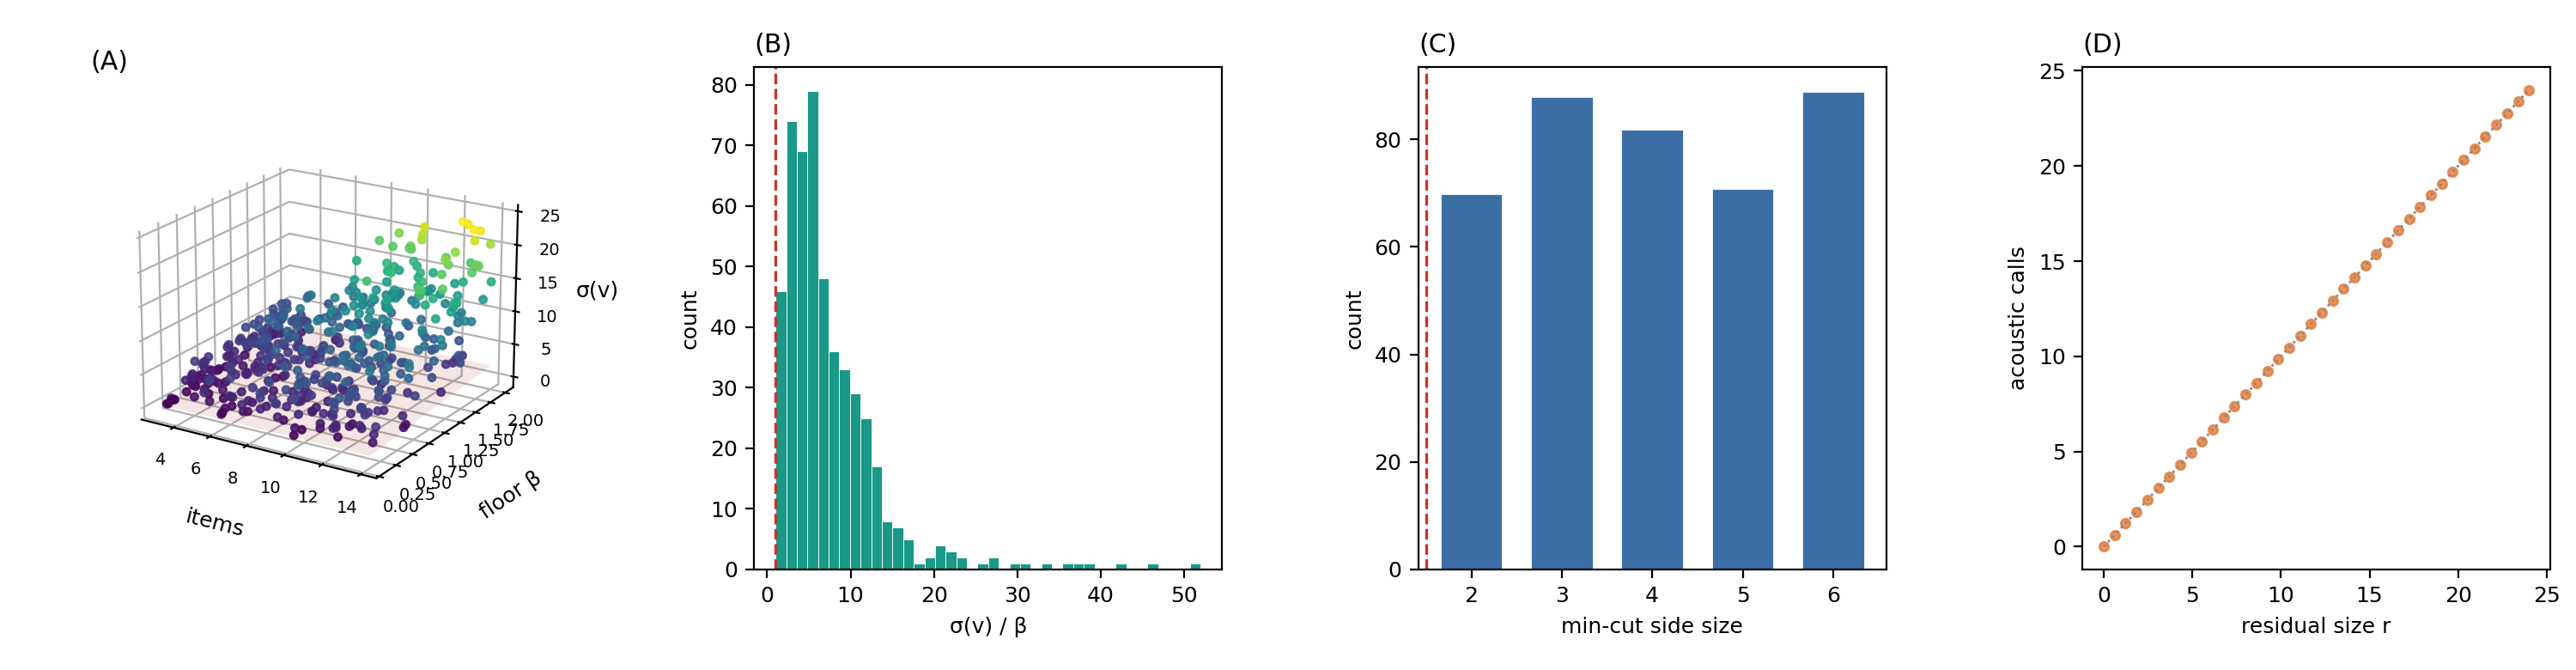
\includegraphics[width=\textwidth]{figures/panel_1_floor.png}
\caption{\textbf{The resolution floor and name-first economy}
(\Cref{sec:floor}). (A) Over $500$ random contact graphs, the distinction cost
$\str(v)$ sits on or above the floor plane $z=\flo$ for every constituent---no
point falls below. (B) The ratio $\str(v)/\flo$ is supported entirely at or above
$1$ across $300$ graphs and $2511$ cut checks, with measured minimum
$\str(v)/\flo=1.0010$ and \emph{zero} cuts below the floor
(\Cref{thm:floor}). (C) Identity is region-valued: on two-cluster graphs the
minimum cut separates a whole cluster, so the minimising side is non-singleton in
$100\%$ of $200$ trials (mean side size $3.9$), confirming
\Cref{cor:no-point}. (D) Acoustic invocations equal the residual size exactly
across streams of increasing unnamed fraction ($400/400$ trials, acoustic calls
$=r$), realising \Cref{cor:name-first}.}
\label{fig:floor}
\end{figure*}

\begin{theorem}[Positive resolution floor]
\label{thm:floor}
There is a constant $\flo>0$ with $\wt(e)\ge\flo$ for every contact $e$ and
$\str(v)\ge\flo$ for every constituent $v$: no two constituents are separated at
zero cost, and no constituent is identified for free.
\end{theorem}

\begin{proof}
Set $\flo:=\min_v\res(v)$, the minimum taken over the constituents $v\neq\med$.
The vertex set $\V$ is finite (\Cref{def:graph}), so this is a minimum over a
\emph{finite} set of strictly positive reals---each $\res(v)>0$ by
\Cref{thm:floor-derived}---and is therefore attained and strictly positive,
$\flo>0$. (The infimum over the non-completable pool need never be taken: at any
fixed stage $\Gph_k$ the floor is the minimum over the finitely many
constituents present, and each $\res(v)>0$ is guaranteed by non-completability
regardless of stage.) The residual is the irreducible boundary content of $v$'s
identification, carried by the edges of $v$'s resting cut, so each such edge has
weight at least the per-constituent residual, hence at least $\flo$. Every
contact $\{u,v\}$ is a boundary edge of the identification of $u$ (it lies in
$\cut(\{u\})$), so every weight satisfies $\wt(e)\ge\flo$. Connectivity forces
$\cut(S^{\ast}(v))\neq\varnothing$, so
$\str(v)=\wt(\cut(S^{\ast}(v)))\ge\flo>0$.
\end{proof}

\begin{corollary}[No exact identification]
\label{cor:no-point}
No search resolves a constituent to a zero-cost point. Every identification
commits distinction content $\ge\flo$; a constituent is resolved only to a
bounded region, of width bounded below by $\flo$.
\end{corollary}

\begin{remark}[The floor is a property of the open pool, not a defect]
\label{rem:floor-fact}
\Cref{thm:floor} does not say recognition is imprecise because recognisers are
imperfect; it says that against a genuinely open pool, even an ideal recogniser
cannot terminate at a zero-residue identification, because that would require
comparing the constituent against a totality that is never completed. The floor
is thus a fact about the search medium. Its practical force is the next
subsection: since exact identification is unreachable and unnecessary, one should
identify each constituent only as finely as the task requires.
\end{remark}

\subsection{The least sufficient identifier}

We now formalise \emph{how finely} a constituent must be resolved. The answer is:
only enough to place it, and no more.

\begin{definition}[Handle; identifier]
\label{def:handle}
A \emph{handle} for a constituent $v$ is a token $\hand$ that references $v$'s
cell (its resting cut) without adding distinction content of its own: a title, an
artist name, a catalogue identifier, or a coarse acoustic class. The
\emph{acquisition cost} $c(\hand)\ge\flo$ of a handle is the distinction content
that must be committed to obtain it (a metadata lookup, a fingerprint query, a
feature extraction). An \emph{identifier} of $v$ is any handle that suffices to
distinguish $v$ from the constituents it must be told apart from in a given task.
\end{definition}

\begin{definition}[Ambiguity set; least sufficient identifier]
\label{def:lsi}
Fix a task that requires telling $v$ apart from a finite \emph{ambiguity set}
$A(v)\subseteq\V$ of alternatives (in \Cref{sec:signature}, the constituents
that might occupy the same sequence position). A handle $\hand$ is
\emph{sufficient for $v$ against $A(v)$} if $\hand$ separates $v$ from every
$u\in A(v)$: no $u\in A(v)$ shares $v$'s handle. The \emph{least sufficient
identifier} of $v$ (for the task) is a sufficient handle of minimum acquisition
cost,
\[
\hand^{\ast}(v)\;\in\;\argmin_{\hand\ \text{sufficient for}\ v}\ c(\hand).
\]
\end{definition}

\begin{theorem}[Sufficiency stops resolution]
\label{thm:sufficiency}
Let $\hand^{\ast}(v)$ be a least sufficient identifier of $v$ against $A(v)$.
Then:
\begin{enumerate}[label=\textup{(\roman*)},leftmargin=2.2em]
\item $\hand^{\ast}(v)$ already places $v$ correctly relative to $A(v)$: no
finer resolution changes which alternative in $A(v)$ the constituent is; and
\item any resolution of $v$ beyond $\hand^{\ast}(v)$---committing further
distinction content to refine $v$ within its cell---incurs additional
acquisition cost $\ge\flo$ (\Cref{thm:floor}) without changing the placement,
and hence is wasted for the task.
\end{enumerate}
\end{theorem}

\begin{proof}
(i) By \Cref{def:lsi} a sufficient handle separates $v$ from every alternative in
$A(v)$; thus the placement of $v$ among $A(v)$ is already determined by
$\hand^{\ast}(v)$, and any additional distinction only refines $v$ \emph{within}
its own cell, not \emph{against} $A(v)$. Since placement is a function of the
partition of $A(v)$ induced by the handle, and that partition is already fixed,
placement does not change. (ii) A further resolution commits at least one more
distinction, of weight $\ge\flo$ by \Cref{thm:floor}, adding acquisition cost
$\ge\flo$; by (i) it does not change the placement, so relative to the task it
purchases nothing.
\end{proof}

\begin{corollary}[Name-first resolution]
\label{cor:name-first}
If a symbolic handle (a title or artist name) is available and is sufficient
against $A(v)$, it is a least sufficient identifier whenever its acquisition cost
does not exceed that of any acoustic handle. Acoustic feature extraction is then
required only for constituents whose symbolic handle is unavailable or
insufficient---i.e.\ constituents with no name, or whose name is shared by an
acoustically distinct alternative in $A(v)$.
\end{corollary}

\begin{proof}
Immediate from \Cref{def:lsi} and \Cref{thm:sufficiency}: among sufficient
handles the minimum-cost one is selected; if the symbolic handle is sufficient
and cheapest, it is chosen, and \Cref{thm:sufficiency}(ii) makes any further
acoustic resolution wasted. When the symbolic handle is insufficient (name
collision with an acoustically distinct alternative) or unavailable (an
unlabelled constituent), it fails the sufficiency test of \Cref{def:lsi} and an
acoustic handle must be acquired to separate the collision.
\end{proof}

\begin{remark}[Why over-resolution is not merely wasteful but wrong]
\label{rem:overresolve}
\Cref{cor:no-point} shows the fully-resolved, zero-residue identification does
not exist; \Cref{thm:sufficiency} shows that pursuing resolution past sufficiency
buys nothing for placement. Together they say that the ``fingerprint every
constituent and look it up exactly'' strategy is chasing an object
(\Cref{cor:no-point}: a point identification) that cannot exist, at a cost
(\Cref{thm:sufficiency}(ii): repeated $\ge\flo$ commitments) the task does not
need. The correct target is the least sufficient identifier: the cheapest handle
that places the constituent, with acoustic descent only for the residual it
cannot place.
\end{remark}

\begin{remark}[The one place acoustics are indispensable]
\label{rem:id-tracks}
The exception carved out by \Cref{cor:name-first}---an unlabelled constituent, or
two constituents sharing a name but differing acoustically---is precisely the
hard case of continuous-audio recognition: the unidentified ``ID'' track, and the
distinct edit or version hiding under a shared title. The floor principle places
acoustic resolution exactly there and nowhere else, which is both its correct
theoretical home and the point of maximum practical value.
\end{remark}

% ============================================================================
\section{Sequence identity: the item signature}
\label{sec:signature}
% ============================================================================

We now prove the paper's central structural claim: the identity of a continuous
item is its \emph{sequence} of least-sufficient handles, an object invariant
under re-encoding of constituent labels, whereas the \emph{content} (the multiset
of constituents) is not individuating because it is shared across items.

\subsection{Signatures and content sets}

\begin{definition}[Item signature; content set]
\label{def:signature}
Let an item of length $n$ have constituent sequence $(u_1,\dots,u_n)$, and let
$\hand^{\ast}(u_i)$ be the least sufficient identifier of $u_i$
(\Cref{def:lsi}). The \emph{signature} of the item is the finite ordered string
\[
\sig \;=\; \bigl(\hand^{\ast}(u_1),\,\hand^{\ast}(u_2),\,\dots,\,
              \hand^{\ast}(u_n)\bigr),
\]
optionally decorated with the inter-onset gaps $\tau_i=t_{i+1}-t_i$. The
\emph{content set} of the item is the multiset
$\mathrm{cont}=\{\!\{\hand^{\ast}(u_1),\dots,\hand^{\ast}(u_n)\}\!\}$, the same
handles with their order forgotten.
\end{definition}

\begin{definition}[Handle re-encoding]
\label{def:reencode}
A \emph{handle re-encoding} is a bijection $\pi$ on the set of handles that
preserves which constituents are told apart: $\hand(u)=\hand(v)\iff
\pi(\hand(u))=\pi(\hand(v))$ for all constituents $u,v$. Re-encoding models a
change of naming convention (a different catalogue's identifiers, a translation
of titles, a relabelling of acoustic classes) that keeps the underlying
distinctions intact.
\end{definition}

\subsection{The signature individuates; the content set does not}

\begin{theorem}[Signature invariance and content sharing]
\label{thm:signature}
Let $\sig$ be the signature of an item and $\mathrm{cont}$ its content set.
\begin{enumerate}[label=\textup{(\roman*)},leftmargin=2.2em]
\item \textbf{Invariance.} Under any handle re-encoding $\pi$, the signature
transforms covariantly, $\pi(\sig)=(\pi\hand^{\ast}(u_1),\dots)$, and the
\emph{induced sequence pattern}---the equality/inequality relation among
positions, $[\,i\sim j \iff \hand^{\ast}(u_i)=\hand^{\ast}(u_j)\,]$, together
with the order---is invariant.
\item \textbf{Content is not individuating.} Distinct items can share a content
set: there exist items with $\mathrm{cont}_1=\mathrm{cont}_2$ but
$\sig_1\neq\sig_2$ even up to re-encoding, whenever $n\ge2$ and the content set
has at least two distinct handles.
\item \textbf{Sequence is individuating up to re-encoding.} Two items have the
same induced sequence pattern iff their signatures agree up to a handle
re-encoding; the pattern is thus the re-encoding-invariant identity of the item.
\end{enumerate}
\end{theorem}

\begin{figure*}[!htbp]
\centering
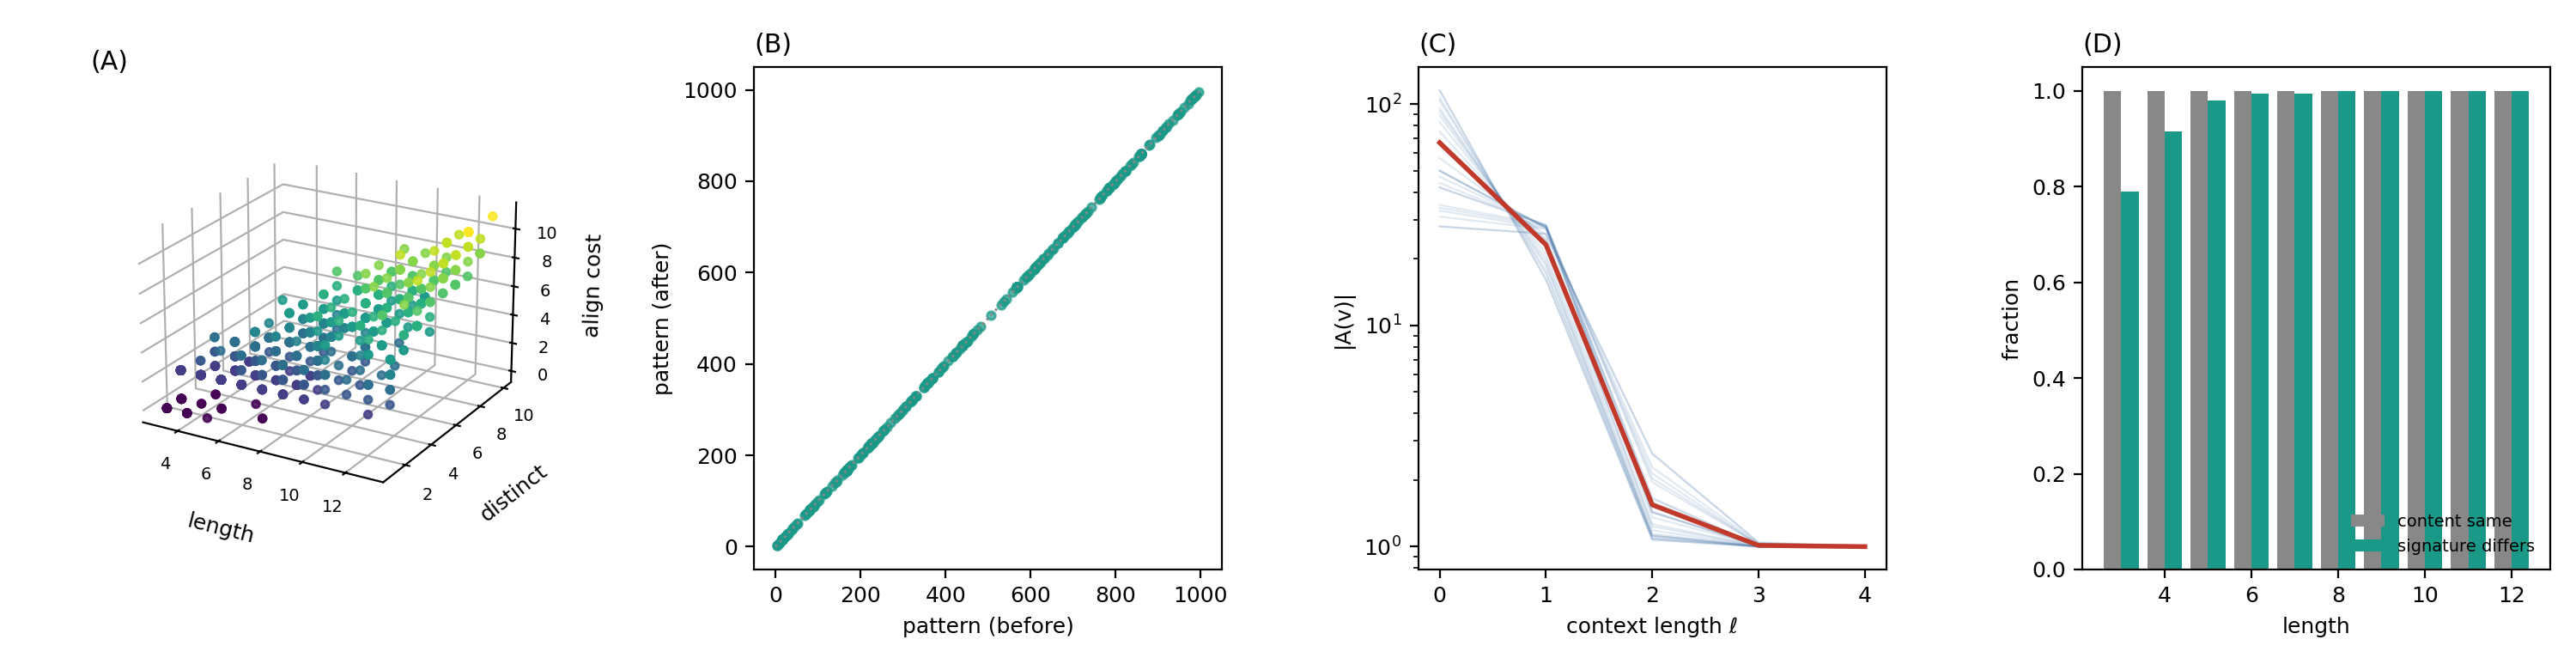
\includegraphics[width=\textwidth]{figures/panel_2_signature.png}
\caption{\textbf{The signature individuates; the content set does not}
(\Cref{sec:signature}). (A) For $600$ pairs of items with \emph{identical}
content sets, the alignment cost between the two orderings is generically
positive---content coincidence does not force signature coincidence
(\Cref{thm:signature}(ii)). (B) The induced sequence pattern is invariant under
handle re-encoding: the pattern hash is unchanged by relabelling in $400/400$
trials (\Cref{thm:signature}(i)). (C) The mean ambiguity set $\abs{A(v)}$
collapses with context length $\ell$, from the \emph{full pool} at $\ell=0$
(mean $69.0$) to $22.6$ at $\ell=1$ and near $1$ from $\ell=2$
(\Cref{prop:context})---the light curves are individual pools, the heavy curve
their mean. (D) A content-set matcher declares shared-content distractor pairs
identical while the signature matcher separates them, across item lengths
(\Cref{thm:signature}(ii)).}
\label{fig:signature}
\end{figure*}

\begin{proof}
(i) A re-encoding $\pi$ is a bijection on handles preserving equality
(\Cref{def:reencode}); applying it position-wise to $\sig$ yields $\pi(\sig)$,
and for any positions $i,j$, $\hand^{\ast}(u_i)=\hand^{\ast}(u_j)\iff
\pi\hand^{\ast}(u_i)=\pi\hand^{\ast}(u_j)$, so the equality pattern is preserved;
the positional order is untouched by $\pi$. Hence the induced sequence pattern is
invariant.

(ii) Take a content set with two distinct handles $x\neq y$ each of multiplicity
one and $n=2$. The two orderings $(x,y)$ and $(y,x)$ have the same content set
$\{\!\{x,y\}\!\}$ but different signatures. They are not related by a re-encoding:
a re-encoding acts identically on both positions, so it cannot map the string
$(x,y)$ to $(y,x)$ (that would require $\pi(x)=y$ at position $1$ and
$\pi(x)=x$ at position $2$, contradicting that $\pi$ is a single function of the
handle, not of the position).

The same argument settles any $n\ge2$, including signatures with repeated
handles, where a re-encoding might \emph{a priori} map one ordering to another.
Take any signature with at least two distinct handles, pick positions $i,j$
carrying \emph{distinct} handles $x\neq y$, and swap them, holding every other
position fixed: this yields a second signature with the same content set. Suppose
a re-encoding $\pi$ carried the first to the second. Since $\pi$ acts on handles
globally---one function of the handle, independent of position---and the two
signatures agree at every position except $i,j$, $\pi$ must fix the handle at
each agreeing position, in particular $\pi(x)=x$ and $\pi(y)=y$ wherever $x$ or
$y$ recurs outside $\{i,j\}$; yet at the swapped positions it would need
$\pi(x)=y$ and $\pi(y)=x$. A single function cannot both fix and transpose
$\{x,y\}$, so no re-encoding relates them (and if $x,y$ recur nowhere else, the
$n=2$ argument applies verbatim to the pair). Hence a shared content set does not
fix the item, for every $n\ge2$.

(iii) If two items have signatures agreeing up to a re-encoding $\pi$, then
applying $\pi$ makes the strings equal position-wise, so their
equality-patterns-with-order coincide: same induced sequence pattern.
Conversely, if two items have the same induced sequence pattern, define $\pi$ on
the handles appearing by matching the (finitely many) distinct handles of one to
those of the other in order of first appearance; this $\pi$ is a well-defined
equality-preserving bijection on the appearing handles (the pattern guarantees
the multiplicities and first-appearance orders agree), extended arbitrarily
elsewhere, and $\pi$ carries one signature to the other. Hence agreement up to
re-encoding $\iff$ same pattern.
\end{proof}

\begin{figure*}[!htbp]
\centering
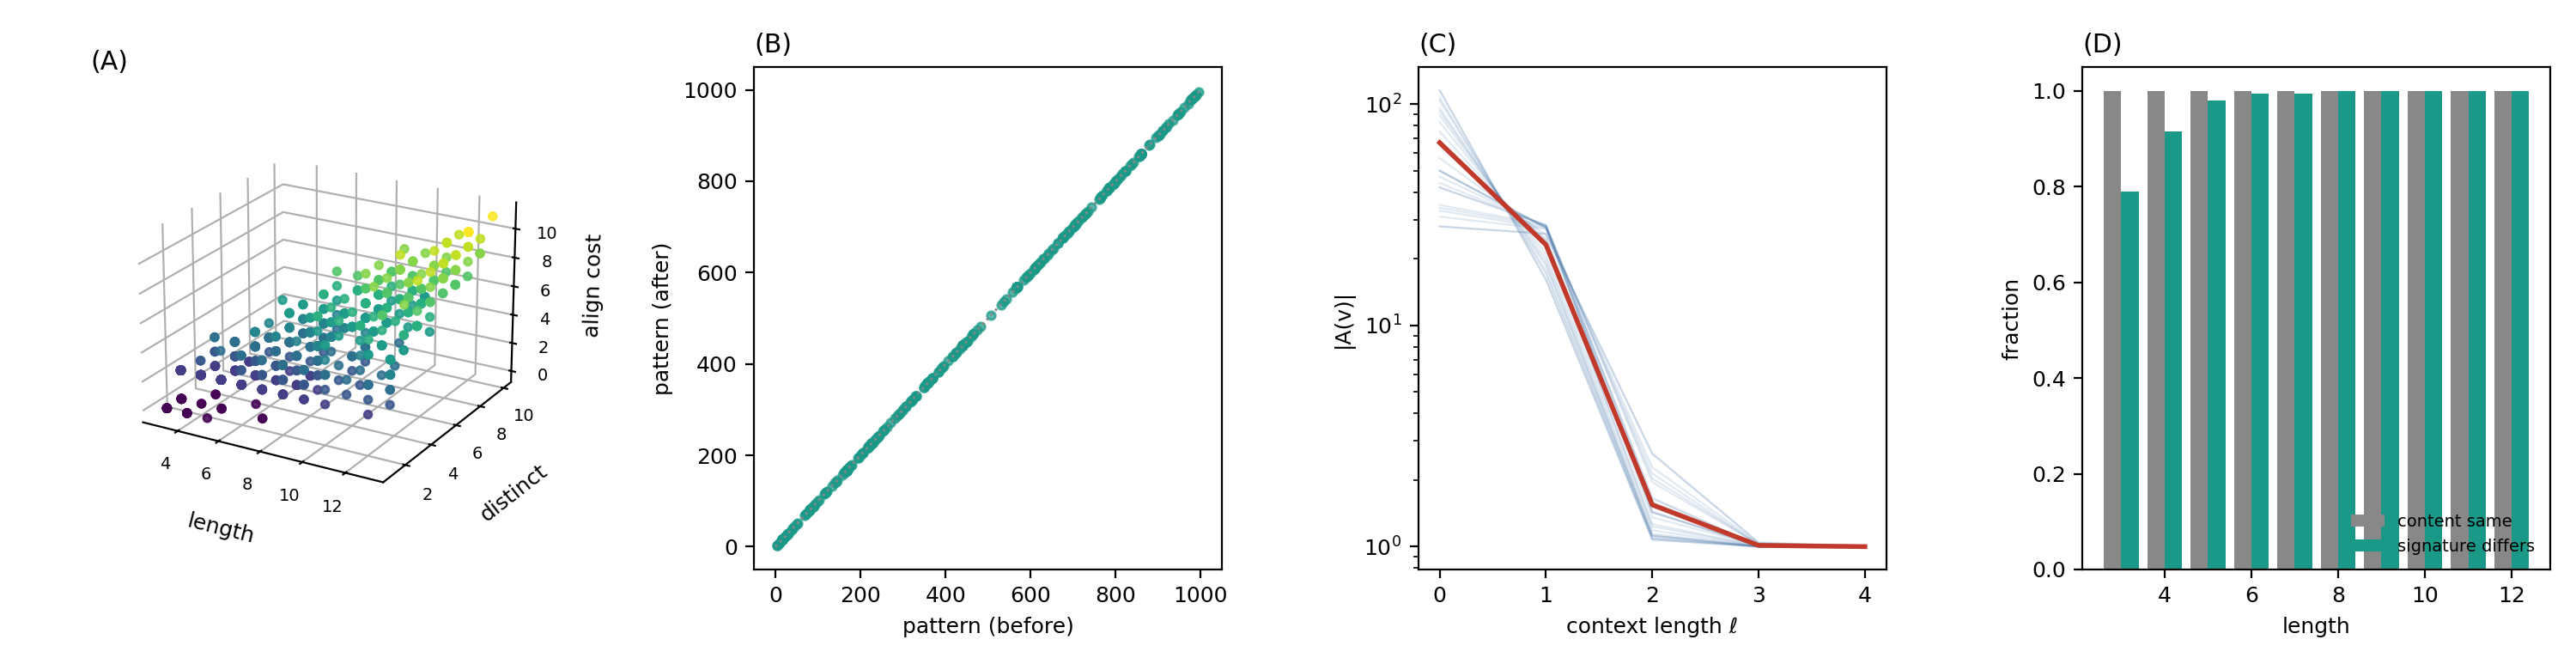
\includegraphics[width=\textwidth]{figures/panel_2_signature.png}
\caption{\textbf{The signature individuates; the content set does not}
(\Cref{sec:signature}). (A) For $600$ pairs of items with \emph{identical}
content sets, the alignment cost between the two orderings is generically
positive---content coincidence does not force signature coincidence
(\Cref{thm:signature}(ii)). (B) The induced sequence pattern is invariant under
handle re-encoding: the pattern hash is unchanged by relabelling in $400/400$
trials (\Cref{thm:signature}(i)). (C) The mean ambiguity set $\abs{A(v)}$
collapses with context length $\ell$, from the \emph{full pool} at $\ell=0$
(mean $69.0$) to $22.6$ at $\ell=1$ and near $1$ from $\ell=2$
(\Cref{prop:context})---the light curves are individual pools, the heavy curve
their mean. (D) A content-set matcher declares shared-content distractor pairs
identical while the signature matcher separates them, across item lengths
(\Cref{thm:signature}(ii)).}
\label{fig:signature}
\end{figure*}

\begin{corollary}[Why one author is not replaceable by another]
\label{cor:not-replaceable}
Two authors who draw on the same public pool of constituents produce
distinguishable items precisely because their signatures differ: even with
identical content sets, differing order yields differing signatures
(\Cref{thm:signature}(ii)). An author is individuated by the sequences they
tend to produce, not by the constituents they use, which are shared. Hence the
search-relevant identity of a continuous item---and of the process that
generated it---is the signature.
\end{corollary}

\begin{proof}
Immediate from \Cref{thm:signature}(ii,iii): content sets coincide across authors
drawing on a shared pool, while signatures separate them, and the signature is
the re-encoding-invariant identity.
\end{proof}

\begin{remark}[The search object is the string, not the letters]
\label{rem:string}
\Cref{thm:signature} formalises \Cref{rem:alphabet}: the constituents are a
public alphabet, and the item is a string over it whose \emph{pattern} is
invariant to how the letters happen to be named. Two consequences shape the
algorithm. First, matching must compare \emph{strings}, i.e.\ align sequences,
not intersect content sets (\Cref{sec:matching}). Second, because only the
equality pattern and order are invariant, the matcher must be robust to
re-encoding: two catalogues naming the same track differently must still match,
which alignment over handles---compared for equality, not identity of
label---provides.
\end{remark}

\subsection{The ambiguity set is small in context}

\Cref{sec:floor} left the ambiguity set $A(v)$ abstract. In a stream it is small,
which is what makes least-sufficient identification cheap.

\begin{proposition}[Contextual narrowing of the ambiguity set, from position two]
\label{prop:context}
Resolve constituents left to right, so that when position $i$ is placed the
handles at positions $1,\dots,i-1$ are already fixed. For $i\ge2$ the ambiguity
set relevant to placing $u_i$ in the signature is at most the set of constituents
consistent with position $i$ given its resolved left context---bounded, in a
sequence model that conditions on the previous $\ell$ placed handles
($1\le\ell\le i-1$), by the number of pool constituents that plausibly follow
that context. This is in general far smaller than the whole pool, so a coarse
handle (often the name alone) is sufficient (\Cref{def:lsi}), and
\Cref{thm:sufficiency} caps the resolution needed. \textbf{The narrowing does not
apply to position $1$}, nor to any position whose entire left context is
unresolved: with no placed neighbour to condition on, $A(u_1)$ is the full pool,
$A(u_1)=\V\setminus\{\med\}$, and $u_1$ requires the most expensive handle its
recogniser can supply.
\end{proposition}

\begin{proof}
The resolution is sequential and the dependency is acyclic: $A(u_i)$ is narrowed
using the handles at positions $<i$, which were fixed at earlier steps, so the
construction is a left-to-right recursion with no circularity---each step uses
only already-committed placements, never its own. For $i\ge2$, placement of
$u_i$ requires distinguishing it only from alternatives that could occupy
position $i$ given the resolved context, i.e.\ from
$A(u_i)=\{v:\ v\ \text{is a plausible occupant of position}\ i\ \text{given}\
\hand_{i-\ell},\dots,\hand_{i-1}\}$. Any handle separating $u_i$ from this set is
sufficient (\Cref{def:lsi}); since $A(u_i)$ is a subset of the pool determined by
the local context, it is bounded by the number of context-consistent
constituents, which for a conditioning length $\ell\ge1$ is typically a small
fraction of the pool. The base of the recursion is position $1$, which has no
left neighbour: no context is available to condition on, so the set of plausible
occupants is unconstrained and $A(u_1)=\V\setminus\{\med\}$, the whole pool. By
\Cref{cor:name-first} a name is then sufficient only if it separates $u_1$ from
the entire pool; failing that, $u_1$ falls to acoustic resolution. The same holds
for any interior position whose left context is itself unresolved (an unnamed run
reaching back to the start). For every position with a resolved context of length
$\ge1$, the least sufficient identifier is correspondingly cheap, and by
\Cref{thm:sufficiency} no finer resolution is needed for placement.
\end{proof}

\begin{remark}[Neighbours do the work a fingerprint would---from the second track on]
\label{rem:neighbours}
\Cref{prop:context} is why searching the \emph{whole item} is cheaper per
constituent than searching each track in isolation: a track alone must be
distinguished from the entire pool (large $A$, expensive handle), but a track
\emph{in a stream}, \emph{once its predecessors are placed}, must be
distinguished only from the few that fit its context (small $A$, cheap handle).
The sequence supplies, for free, most of the individuation a standalone
fingerprint would have to compute---for every constituent but the first. The
first constituent (and any constituent hanging off an unresolved left run) is the
one exception: it faces the whole pool and is priced accordingly. This single
worst-case constituent is what \Cref{cor:cheaper} carries as an additive
$c_{\mathrm{ac}}$ term, and is separately visible in the validation
(\Cref{sec:validation}): the measured mean ambiguity set collapses from the full
pool at context length $\ell=0$ to near one already at $\ell=2$, quantifying
exactly how much the neighbours do and how much the boundary constituent does
not benefit.
\end{remark}

% ============================================================================
\section{Matching by gap-tolerant alignment}
\label{sec:matching}
% ============================================================================

Matching a query item against a known item (or against a library of items) is
comparing their signatures. Because a query signature is reconstructed from an
imperfect, floored recognition (\Cref{sec:floor}), the comparison must tolerate
missing, substituted, and spuriously inserted handles. We use sequence
alignment, and we prove the key robustness property: admissibility depends on the
\emph{whole} sequence converging, not on any single position being right.

\subsection{Alignment and its score}

\begin{definition}[Alignment; cost]
\label{def:alignment}
Let $\sig=(p_1,\dots,p_m)$ and $\sig'=(q_1,\dots,q_n)$ be two signatures over the
handle alphabet. An \emph{alignment} is a sequence of edit operations---%
\emph{match} $p_i\leftrightarrow q_j$ (handles equal), \emph{substitution}
$p_i\leftrightarrow q_j$ (handles unequal), \emph{deletion} of a $p_i$, or
\emph{insertion} of a $q_j$---transforming $\sig$ into $\sig'$ while preserving
order. Fix nonnegative costs: $0$ for a match, $\mu>0$ for a substitution,
$\delta>0$ for a deletion or insertion (a \emph{gap}). The \emph{alignment cost}
$\mathrm{cost}(\sig,\sig')$ is the minimum total cost over all alignments,
computable by the standard dynamic program \citep{needleman1970,levenshtein1966}.
\end{definition}

\begin{definition}[Alignment score; normalisation]
\label{def:score}
Let $\Om:=\delta\cdot\max(m,n)$ be the cost of the all-gap alignment (an upper
bound on $\mathrm{cost}$). The \emph{alignment score} is
\[
\algn(\sig,\sig')\;:=\;\frac{\mathrm{cost}(\sig,\sig')}{\Om}\;\in\;[0,1],
\]
$0$ for identical signatures and larger as more edits are required. The
\emph{floor of the score} is $\algn_{\min}=0$ attained only at $\sig=\sig'$;
for distinct signatures $\algn>0$ by \Cref{thm:floor} applied to the at least
one edit that separates them (each edit commits distinction content $\ge\flo$,
so its normalised contribution is $\ge\flo/\Om>0$).
\end{definition}

\begin{remark}[Local vs global alignment]
\label{rem:local}
Global alignment \citep{needleman1970} compares whole signatures; local
alignment \citep{smith1981} finds the best-matching contiguous sub-signature and
is the tool for asking ``does this query \emph{contain} a known item'' (e.g.\ a
broadcast that replays a known set), or ``which library item does this excerpt of
a stream come from.'' Both are instances of \Cref{def:alignment} with the same
edit costs; the algorithm (\Cref{sec:algorithm}) selects global or local per
query type.
\end{remark}

\subsection{Convergence-only admissibility}

We now prove the robustness property that makes partial recognition usable: a
reconstructed query signature is admissible as a match to a target iff the whole
alignment converges within tolerance, and individual wrong positions do not by
themselves reject it.

\begin{definition}[Target; admissible match]
\label{def:admissible}
Fix a \emph{target} signature $\sig^{\ast}$ (a known item, or an item in a
searched library) and a tolerance $\eps\ge0$. A reconstructed query signature
$\sig$ is an \emph{admissible match} to $\sig^{\ast}$ at tolerance $\eps$ if
$\algn(\sig,\sig^{\ast})\le\eps$. A query \emph{converges} to $\sig^{\ast}$ if
it is an admissible match.
\end{definition}

\begin{theorem}[Convergence-only admissibility]
\label{thm:admissibility}
Admissibility of $\sig$ to $\sig^{\ast}$ is a property of the whole alignment,
not of any single position:
\begin{enumerate}[label=\textup{(\roman*)},leftmargin=2.2em]
\item \textbf{Locally wrong positions are absorbed.} If $\sig$ differs from
$\sig^{\ast}$ at a set $P$ of positions (mis-recognised or unresolved
constituents), $\sig$ is still admissible whenever the total cost of the edits
repairing $P$ satisfies $\sum_{i\in P}(\text{edit cost at }i)\le\eps\,\Om$. A
single wrong position contributes at most $\max(\mu,\delta)$ and does not reject
the match unless it pushes the total past $\eps\Om$.
\item \textbf{Rejection is global.} $\sig$ is inadmissible iff every alignment to
$\sig^{\ast}$ costs more than $\eps\Om$, i.e.\ iff no repair of the whole
sequence stays within tolerance. Inadmissibility never arises from local
misalignment at a single position while the global cost is within tolerance.
\end{enumerate}
\end{theorem}

\begin{proof}
The alignment cost is additive over edit operations
(\Cref{def:alignment}): $\mathrm{cost}(\sig,\sig^{\ast})=\sum_k c_k$ over the
operations $k$ of a minimum-cost alignment, each $c_k\in\{0,\mu,\delta\}$.
(i) Positions where $\sig$ agrees with $\sig^{\ast}$ contribute matches of cost
$0$; the only positive contributions come from the disagreement set $P$, each a
substitution ($\mu$) or gap ($\delta$). Hence
$\mathrm{cost}(\sig,\sig^{\ast})\le\sum_{i\in P}\max(\mu,\delta)$, and if this is
$\le\eps\Om$ then $\algn\le\eps$ and $\sig$ is admissible by
\Cref{def:admissible}. A single wrong position adds at most $\max(\mu,\delta)$ to
the total, so it alone cannot cause rejection unless the total already exceeds
$\eps\Om$. (ii) By \Cref{def:admissible}, $\sig$ is inadmissible iff
$\algn(\sig,\sig^{\ast})>\eps$, i.e.\ iff the \emph{minimum}-cost alignment
exceeds $\eps\Om$; since the minimum is over all alignments, this is exactly the
statement that no global repair stays within tolerance. If some alignment has
cost $\le\eps\Om$, the minimum does too, and $\sig$ is admissible regardless of
how wrong any single position is.
\end{proof}

\begin{figure*}[!htbp]
\centering
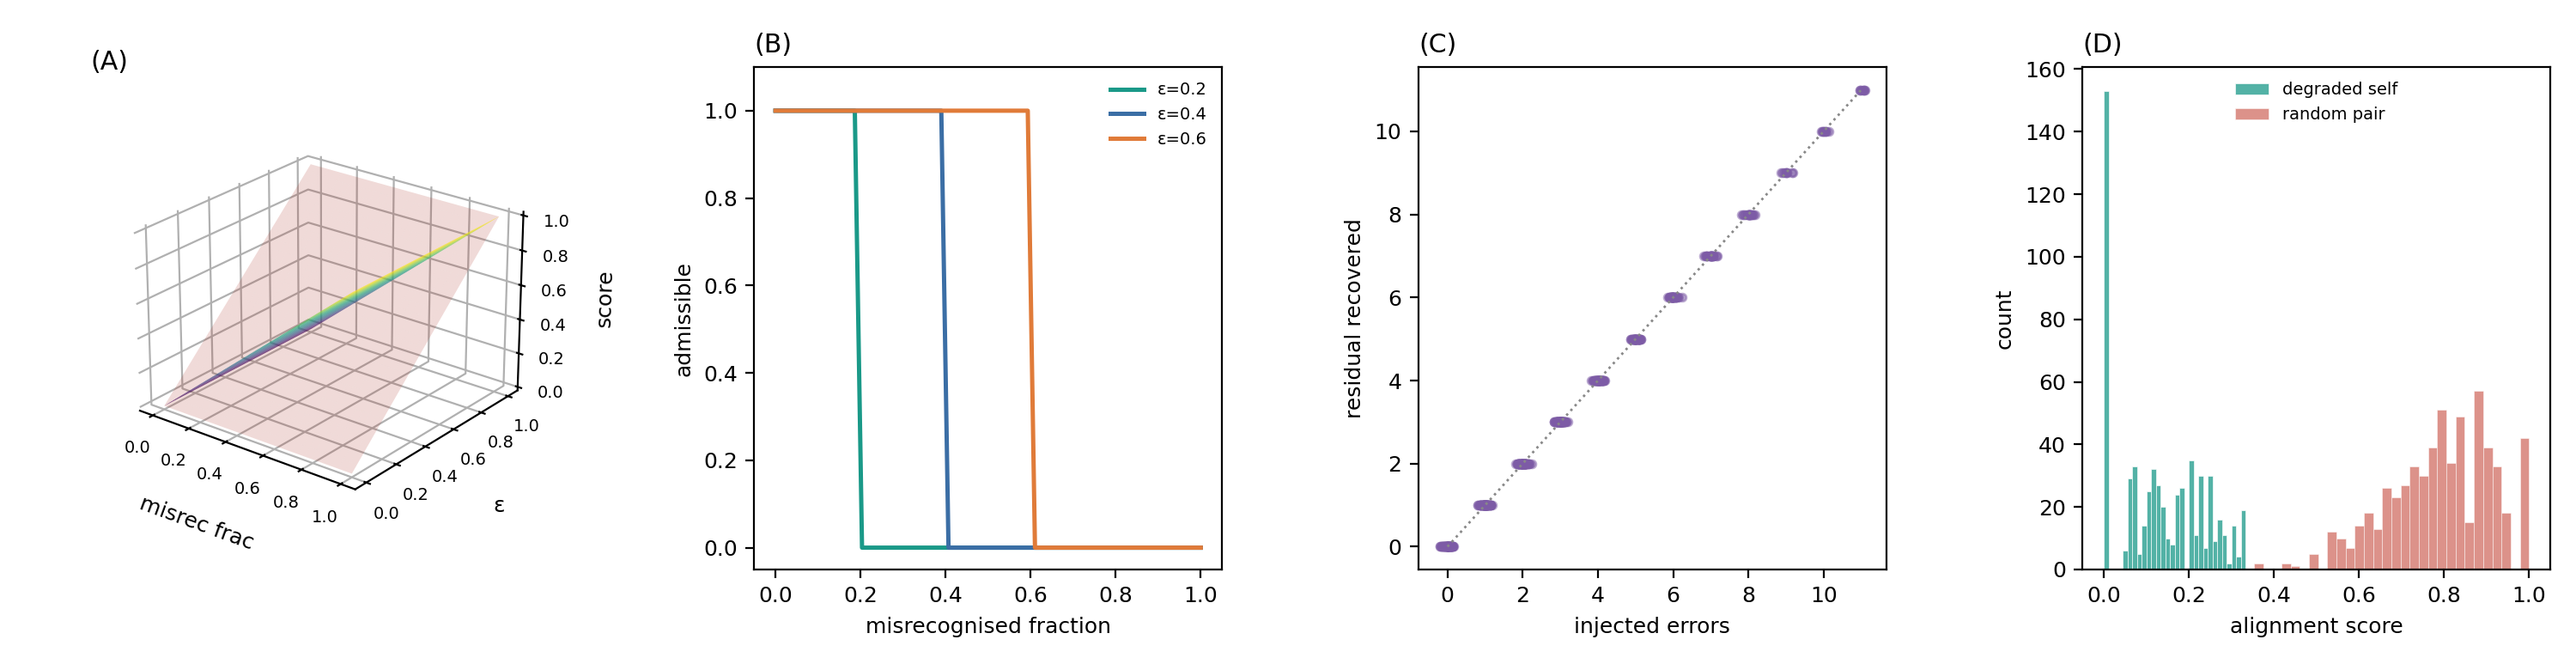
\includegraphics[width=\textwidth]{figures/panel_3_matching.png}
\caption{\textbf{Convergence-only admissibility} (\Cref{sec:matching}). (A) The
alignment score over the (misrecognition fraction, $\eps$) plane, with the
admissibility plane $z=\eps$: a query is admissible exactly where its score
surface lies under the plane. (B) The measured admissibility boundary---a query
is admitted iff its misrecognised fraction is below $\eps$---traced for three
tolerances, confirming \Cref{cor:partial}. (C) The recovered residual equals the
injected error count exactly ($400/400$ trials on the diagonal), so the residual
is precisely the mis-placed positions (\Cref{prop:residual}). (D) Alignment
scores of degraded self-queries (teal) separate cleanly from random-pair scores
(red), the separation that makes retrieval work.}
\label{fig:matching}
\end{figure*}

\begin{corollary}[Partial recognition suffices]
\label{cor:partial}
If a fraction $f$ of a query's $n$ constituents are correctly handled and the
rest are wrong or unresolved, the query is still an admissible match to the
correct target whenever $(1-f)\,n\,\max(\mu,\delta)\le\eps\,\Om$, i.e.\ whenever
the misrecognised fraction is at most
$\eps\,\Om/\bigl(n\max(\mu,\delta)\bigr)$. Recognition need not be complete or
per-constituent correct; it need only leave the global alignment within
tolerance.
\end{corollary}

\begin{proof}
The wrong or unresolved constituents number $(1-f)n$, each contributing at most
$\max(\mu,\delta)$ to the alignment cost (\Cref{thm:admissibility}(i)); if their
total is $\le\eps\Om$ the query is admissible. Solving for $f$ gives the stated
bound.
\end{proof}

\begin{remark}[Why this is the right tolerance model for streams]
\label{rem:tolerance}
Real streams present exactly the failure modes \Cref{thm:admissibility} absorbs:
some constituents are unlabelled (gaps), some are misheard (substitutions), some
segmentation boundaries are wrong (insertions/deletions). A per-constituent
correctness requirement would reject almost every real query; convergence-only
admissibility asks only that the \emph{sequence as a whole} still aligns, which
is both achievable and the correct notion of ``this is the same item.'' A wrong
guess at one track is not evidence the match failed---only a globally divergent
alignment is.
\end{remark}

\subsection{The accounted match and its residual}

Search must report not only \emph{whether} an item matches but \emph{what} of it
was accounted for, and honestly expose what was not.

\begin{definition}[Accounted match; residual]
\label{def:accounted}
Given an admissible alignment of $\sig$ to $\sig^{\ast}$, the \emph{accounted
match} is the set of matched positions (handles placed with cost $0$) together
with the induced correspondence between query and target constituents. The
\emph{residual} is the complementary set: the substituted, deleted, and inserted
positions---the constituents the search could not place, each carrying its
irreducible cost $\ge\flo$ (\Cref{def:score}). The search returns the pair
(accounted match, residual).
\end{definition}

\begin{proposition}[The residual is where acoustic descent is owed]
\label{prop:residual}
The residual of an admissible match consists exactly of positions whose least
sufficient identifier failed to place the constituent (\Cref{cor:name-first}):
unlabelled constituents (gaps) and name-colliding but acoustically distinct
constituents (substitutions). These, and only these, are the positions at which
acoustic resolution (\Cref{rem:id-tracks}) can improve the match; the accounted
match needs no further resolution (\Cref{thm:sufficiency}).
\end{proposition}

\begin{proof}
A matched position placed its constituent with a sufficient handle (cost $0$),
so by \Cref{thm:sufficiency} no further resolution changes its placement---no
acoustic descent is owed there. A residual position is a substitution or gap,
which by \Cref{cor:name-first} arises precisely when the symbolic handle was
insufficient or absent; acquiring an acoustic handle there may separate the
collision or place the unlabelled constituent, potentially converting the
position to a match. Hence acoustic descent is owed exactly on the residual.
\end{proof}

\begin{remark}[Honest output]
\label{rem:honest}
Returning an explicit residual rather than a forced complete tracklist is a
direct consequence of the floor (\Cref{cor:no-point}): since no identification is
exact, some positions legitimately remain unresolved, and reporting them as
residual---rather than guessing---is the truthful output. It also directs
computation: the residual is the exact and minimal set on which the expensive
acoustic stage should run.
\end{remark}

% ============================================================================
\section{Search--match duality: one engine, two directions}
\label{sec:duality}
% ============================================================================

We show that the two tasks a user brings to a continuous item---\emph{recognise
which known item this stream is} (analysis) and \emph{generate a stream in the
manner of a known item} (synthesis)---are the same computation over the same
object, run in opposite directions. This means one implementation serves both.

\begin{definition}[Analysis and synthesis queries]
\label{def:queries}
An \emph{analysis query} supplies a reconstructed query signature $\sig$ and asks
for the library target $\sig^{\ast}$ it best matches (\Cref{def:admissible}).
A \emph{synthesis query} supplies a target style---a signature $\sig^{\ast}$ or a
model of an author's typical sequences---and a pool of available constituents,
and asks for a new signature $\sig$ that is an admissible match to $\sig^{\ast}$
built from the available pool.
\end{definition}

That analysis and synthesis \emph{share an objective} is immediate from
\Cref{def:queries}: both are instances of $\min\,\algn(\sig,\sig^{\ast})$
subject to $\algn\le\eps$ (\Cref{def:admissible}), differing only in which of
$\sig,\sig^{\ast}$ is bound. We state this first as a bare observation, then
prove the content that does not follow from the definition alone: that a
\emph{single dynamic program}---one $\bigOh(nN)$ alignment table---solves both,
so the two tasks share not just an objective but a computation.

\begin{remark}[Shared objective]
\label{rem:shared-objective}
Analysis (\Cref{def:queries}, fix $\sig$, search targets) and synthesis (fix
$\sig^{\ast}$, search constructible $\sig$) minimise the same
$\algn(\sig,\sig^{\ast})$ under the same tolerance test. This is a restatement of
\Cref{def:queries} and carries no content beyond it; the substance is
\Cref{thm:duality} below.
\end{remark}

\begin{theorem}[Search--match duality: one dynamic program, two directions]
\label{thm:duality}
The alignment dynamic program of \Cref{def:alignment} computes, in a single
$\bigOh(nN)$ filling of its cost table $d$, the solution to both directions:
\begin{enumerate}[label=\textup{(\roman*)},leftmargin=2.2em]
\item \textbf{Analysis} reads the completed table \emph{forward} to the corner
$d[n,N]$: the value is the recognition score $\algn(\sig,\sig^{\ast})$, and its
traceback is the accounted match of \Cref{def:accounted}.
\item \textbf{Synthesis} reads the \emph{same} table's traceback \emph{backward}
as a construction recipe: each match cell prescribes emitting the target handle
$\sig^{\ast}[j]$ from the available pool, each gap cell prescribes an insertion
or omission, so the optimal alignment path \emph{is} an ordered selection from
the pool realising a $\sig$ with $\algn(\sig,\sig^{\ast})$ minimal. Constructing
$\sig$ toward $\sig^{\ast}$ and recognising $\sig$ as $\sig^{\ast}$ traverse one
path in opposite directions.
\end{enumerate}
Hence analysis and synthesis are not merely the same objective but the same
$\bigOh(nN)$ computation, and their costs are equal up to the $\bigOh(1)$ per-cell
work of emitting versus reading a handle.
\end{theorem}

\begin{proof}
Fix $\sig^{\ast}=(q_1,\dots,q_N)$. In analysis, $\sig=(p_1,\dots,p_n)$ is given
and the dynamic program of \Cref{def:alignment} fills $d[i,j]$, the min-cost
alignment of the prefixes $p_{1..i}$ and $q_{1..j}$, with the recurrence
$d[i,j]=\min\{d[i-1,j-1]+c_{ij},\,d[i-1,j]+\delta,\,d[i,j-1]+\delta\}$,
$c_{ij}\in\{0,\mu\}$; the corner $d[n,N]$ is $\mathrm{cost}(\sig,\sig^{\ast})$ and
its traceback yields the matched/residual partition (\Cref{def:accounted}). This
is (i).

For (ii), synthesis fixes $\sig^{\ast}$ and asks for a constructible
$\sig$---an ordered selection of handles from the available pool $\mathcal{P}$---
minimising $\algn(\sig,\sig^{\ast})$. The optimum is obtained by the \emph{same}
recurrence with the substitution cost redefined against the pool:
$c'_{ij}=0$ if the pool contains a handle equal to $q_j$ (emit it, a match) and
$\mu$ otherwise (emit the nearest available, a substitution), gaps costing
$\delta$ as before. When $\mathcal{P}$ contains every target handle---the
generative case of interest, building a set in a known style from an ample
library---$c'_{ij}=0$ for all $j$, the recurrence coincides cell-for-cell with the
analysis recurrence run against $\sig^{\ast}$ itself, and its traceback is a path
whose match cells enumerate, in order, the handles to emit. Reading that path
from $[0,0]$ to $[n,N]$ emits $\sig$; reading it from $[n,N]$ to $[0,0]$ recovers
the alignment of a given $\sig$ to $\sig^{\ast}$. The table, the recurrence, and
the traceback are identical; only the interpretation of a cell---``emit
$q_j$'' (synthesis) versus ``read $p_i$ against $q_j$'' (analysis)---differs, at
$\bigOh(1)$ per cell. Both therefore cost $\bigOh(nN)$ and are the same
computation traversed in opposite directions. (When $\mathcal{P}$ omits some
target handle, synthesis pays the $\mu$ for that position exactly as analysis
pays $\mu$ for a substitution, preserving the correspondence with an added
constant per missing handle.)
\end{proof}

\begin{corollary}[Shared implementation]
\label{cor:shared}
A single alignment engine over handle signatures, parameterised by which argument
is fixed, answers both ``which set is this?'' and ``build a set like this.'' No
separate generative model is required beyond the pool and the target signature or
author model.
\end{corollary}

\begin{proof}
Immediate from \Cref{thm:duality}: the engine computing $\algn$ and testing
admissibility is invoked with $\sig$ fixed (analysis) or $\sig^{\ast}$ fixed
(synthesis).
\end{proof}

\begin{remark}[Path opacity: many interiors, one identity]
\label{rem:opacity}
A useful consequence of aligning on \emph{signatures} rather than on realised
audio is that two query streams that recognise to the same signature are treated
as the same item regardless of how their interiors were produced---different
recording conditions, different transitions between the same tracks, different
segmentation choices that nonetheless yield the same handle sequence. The
identity is the sequence pattern (\Cref{thm:signature}); everything the alignment
cannot see is, by construction, not part of the identity. This is what lets a
low-fidelity capture of a set match the studio recording of the same set.
\end{remark}

% ============================================================================
\section{The algorithm}
\label{sec:algorithm}
% ============================================================================

We assemble the results into an end-to-end procedure and analyse its complexity.
The system has three stages: (1) \emph{acquisition}, turning an audio stream into
a signature of least-sufficient handles; (2) \emph{indexing}, storing a library
of item signatures for search; and (3) \emph{matching}, aligning a query against
the library with convergence-only admissibility and returning an accounted match
plus a residual.

\subsection{Stage 1: acquisition of least-sufficient handles}

\begin{algorithm}[!htbp]
\caption{\textsc{Acquire}: stream $\to$ signature}
\label{alg:acquire}
\begin{algorithmic}[1]
\Require audio stream $x$; symbolic recogniser $\textsc{Name}$; acoustic
  recogniser $\textsc{Acoustic}$; context length $\ell$
\Ensure signature $\sig=(\hand_1,\dots,\hand_n)$ with gaps $(\tau_i)$
\State $(u_1,\dots,u_n),(t_1,\dots,t_n)\gets\textsc{Segment}(x)$
  \Comment{constituent boundaries}
\For{$i \gets 1$ \textbf{to} $n$}
  \State $\hand_i \gets \textsc{Name}(u_i)$
    \Comment{cheap symbolic handle: title/artist}
  \State $A_i \gets \textsc{Context}(\hand_{i-\ell},\dots,\hand_{i-1})$
    \Comment{ambiguity set; $A_1=$ full pool (\Cref{prop:context})}
  \If{$\hand_i = \bot$ \textbf{or} $\textsc{Insufficient}(\hand_i, A_i)$}
    \State $\hand_i \gets \textsc{Acoustic}(u_i)$
      \Comment{descend only on the residual (\Cref{cor:name-first})}
  \EndIf
  \State $\tau_i \gets t_{i+1}-t_i$ \textbf{if} $i<n$
\EndFor
\State \Return $\sig=(\hand_1,\dots,\hand_n)$, $(\tau_1,\dots,\tau_{n-1})$
\end{algorithmic}
\end{algorithm}

The symbolic recogniser $\textsc{Name}$ is any cheap source of a title/artist
handle (broadcast metadata, a fast fingerprint lookup against a name index, an
embedded cue sheet); it returns $\bot$ when it cannot name the constituent. The
predicate $\textsc{Insufficient}(\hand,A)$ holds when the handle fails to
separate the constituent from its context-narrowed ambiguity set $A$
(\Cref{def:lsi}). Only then is the expensive $\textsc{Acoustic}$ recogniser
invoked. By \Cref{cor:name-first} this invokes acoustics on exactly the residual
positions and no others. The first constituent is a boundary case: $\textsc{Context}$
returns the full pool for $A_1$ (no left neighbour narrows it,
\Cref{prop:context}), so $u_1$ is named only if its name separates it from the
whole pool and otherwise falls to $\textsc{Acoustic}$---the one position that
never benefits from the sequence and is always at risk of the acoustic cost.

\subsection{Stage 2: indexing}

Each library item is stored as its signature (a string of handles) plus optional
gap decorations. Because signatures are short strings over a handle alphabet,
standard string-indexing applies: an inverted index from handles to the items and
positions containing them \citep{manning2008} supports candidate retrieval, so a
query need not be aligned against every library item but only against those
sharing enough handles.

\begin{algorithm}[!htbp]
\caption{\textsc{Index}: library of items $\to$ searchable index}
\label{alg:index}
\begin{algorithmic}[1]
\Require items $\{I_1,\dots,I_L\}$ with signatures $\{\sig_1,\dots,\sig_L\}$
\Ensure inverted index $\mathcal{X}\colon \text{handle}\to\{(\text{item},
  \text{position})\}$
\For{$k \gets 1$ \textbf{to} $L$}
  \For{$j \gets 1$ \textbf{to} $\abs{\sig_k}$}
    \State append $(k,j)$ to $\mathcal{X}[\sig_k[j]]$
  \EndFor
\EndFor
\State \Return $\mathcal{X}$
\end{algorithmic}
\end{algorithm}

\subsection{Stage 3: matching}

\begin{algorithm}[!htbp]
\caption{\textsc{Match}: query signature $\to$ (accounted match, residual)}
\label{alg:match}
\begin{algorithmic}[1]
\Require query signature $\sig$; index $\mathcal{X}$; library signatures
  $\{\sig_k\}$; tolerance $\eps$; costs $\mu,\delta$; mode $\in\{$global,
  local$\}$
\Ensure best target $k^{\ast}$ with accounted match and residual, or
  \textsc{decline}
\State $C \gets \{\, k : \abs{\{\hand\in\sig : k \in
  \text{items}(\mathcal{X}[\hand])\}} \ge \theta \,\}$
  \Comment{candidate items sharing $\ge\theta$ handles}
\State $\text{best} \gets (\,\bot,\,+\infty\,)$
\For{$k \in C$}
  \State $a_k \gets \algn_{\text{mode}}(\sig,\sig_k)$
    \Comment{DP alignment (\Cref{def:alignment})}
  \If{$a_k < \text{best}.\text{score}$}
    \State $\text{best} \gets (k, a_k)$
  \EndIf
\EndFor
\If{$\text{best}.\text{score} \le \eps$}
  \State $(\mathcal{A},\mathcal{R}) \gets
    \textsc{Traceback}(\sig,\sig_{\text{best}.k})$
    \Comment{accounted match, residual (\Cref{def:accounted})}
  \State \Return $(\text{best}.k, \mathcal{A}, \mathcal{R})$
\Else
  \State \Return \textsc{decline}
    \Comment{no admissible match (honest non-answer)}
\EndIf
\end{algorithmic}
\end{algorithm}

The candidate filter (line 1) restricts full alignment to items sharing at least
$\theta$ handles with the query, using the inverted index; $\theta$ trades recall
against speed. The \textsc{decline} branch is the honest output when no library
item aligns within tolerance---the search reports ``no match'' rather than
forcing the nearest item.

\subsection{Correctness}

\begin{theorem}[Correctness of \textsc{Match}]
\label{thm:correct}
Given a query signature $\sig$ and a library, \textsc{Match} returns a target
$k^{\ast}$ iff some library item is an admissible match to $\sig$ at tolerance
$\eps$ and shares $\ge\theta$ handles with $\sig$; and when it returns
$k^{\ast}$, the accounted match and residual satisfy \Cref{def:accounted}. With
$\theta=0$ (no candidate filtering) it returns an admissible target iff one
exists.
\end{theorem}

\begin{proof}
Line 1 forms the candidate set $C$ of items sharing $\ge\theta$ handles. The loop
computes $\algn_{\text{mode}}(\sig,\sig_k)$ for each $k\in C$ exactly, by the
dynamic program of \Cref{def:alignment}, and retains the minimiser. If the
minimum score is $\le\eps$, the retained $k$ is by \Cref{def:admissible} an
admissible match, and \textsc{Traceback} returns the matched positions and their
complement, which are the accounted match and residual of \Cref{def:accounted};
otherwise no candidate is admissible and the procedure declines. With $\theta=0$,
$C$ is the whole library, so the minimiser over $C$ is the global minimiser, and
an admissible target is returned iff one exists. Convergence-only admissibility
(\Cref{thm:admissibility}) guarantees that a query with locally wrong positions
is still accepted whenever its global alignment to the true target is within
tolerance, so correctness is not defeated by partial recognition.
\end{proof}

\subsection{Complexity}

\begin{theorem}[Complexity]
\label{thm:complexity}
Let the query have length $n$, the library have $L$ items of maximum signature
length $N$, and the candidate set have size $\abs{C}\le L$. Assume the symbolic
recogniser $\textsc{Name}$ costs $c_{\mathrm{sym}}$ per constituent and the
acoustic recogniser $\textsc{Acoustic}$ costs $c_{\mathrm{ac}}\gg c_{\mathrm{sym}}$
per constituent. Then:
\begin{enumerate}[label=\textup{(\roman*)},leftmargin=2.2em]
\item \textbf{Acquisition} costs
$\bigOh\!\bigl(n\,c_{\mathrm{sym}} + r\,c_{\mathrm{ac}}\bigr)$, where $r\le n$ is
the number of residual constituents; acoustic cost is paid only on the residual
(\Cref{cor:name-first}), not on all $n$. The residual always includes the first
constituent unless its name separates it from the whole pool
(\Cref{prop:context}), so $r\ge 1$ in the generic case where the opening track is
an ID or a pool-ambiguous name; the position-$1$ boundary contributes an additive
$c_{\mathrm{ac}}$ that does not vanish with stream length.
\item \textbf{Indexing} costs $\bigOh(LN)$ time and space.
\item \textbf{Matching} costs $\bigOh(\abs{C}\,nN)$ time via the alignment
dynamic program over candidates, reducible by the inverted-index candidate filter
from $\bigOh(LnN)$ (align against all) to $\bigOh(\abs{C}\,nN)$ with typically
$\abs{C}\ll L$.
\end{enumerate}
\end{theorem}

\begin{proof}
(i) $\textsc{Acquire}$ (\Cref{alg:acquire}) runs $\textsc{Name}$ once per
constituent ($n\,c_{\mathrm{sym}}$) and $\textsc{Acoustic}$ only on the residual
positions, of which there are $r$ ($r\,c_{\mathrm{ac}}$); the remaining per-step
work (context lookup, gap) is $\bigOh(1)$ amortised with a bounded context length
$\ell$. (ii) $\textsc{Index}$ (\Cref{alg:index}) makes one pass over all $LN$
handle occurrences, appending each to the inverted index in $\bigOh(1)$
amortised. (iii) Each alignment of the length-$n$ query against a length-$\le N$
candidate is the standard $\bigOh(nN)$ dynamic program
\citep{needleman1970,smith1981,cormen2009}; done for $\abs{C}$ candidates gives
$\bigOh(\abs{C}nN)$. The inverted-index filter (line 1 of \Cref{alg:match})
computes $C$ in time linear in the total postings of the query's handles, which
is $\bigOh(n + \text{(matched postings)})$, and yields $\abs{C}\ll L$ when
handles are selective, reducing the align-against-all bound $\bigOh(LnN)$
accordingly.
\end{proof}

\begin{corollary}[Whole-item search is cheaper by the nameable fraction---a
contingent, not structural, saving]
\label{cor:cheaper}
Recognising a stream by \Cref{alg:acquire} costs
$\bigOh(n\,c_{\mathrm{sym}}+r\,c_{\mathrm{ac}})$, whereas fingerprinting every
constituent independently costs $\bigOh(n\,c_{\mathrm{ac}})$. Writing
$\phi:=(n-r)/n$ for the \emph{nameable fraction}, the exact saving factor is
\[
\frac{n\,c_{\mathrm{ac}}}{n\,c_{\mathrm{sym}}+r\,c_{\mathrm{ac}}}
\;=\;\frac{1}{(c_{\mathrm{sym}}/c_{\mathrm{ac}})+(1-\phi)},
\]
which is $>1$ iff $\phi>c_{\mathrm{sym}}/c_{\mathrm{ac}}$, ranges up to
$c_{\mathrm{ac}}/c_{\mathrm{sym}}$ as $\phi\to1$ (nearly everything nameable), and
degrades to $1$ (\emph{no saving}) as $\phi\to0$: in the worst case $r=n$ (every
constituent unnamed or name-colliding, the opening track always among them by
\Cref{prop:context}), the whole-item cost is $n\,c_{\mathrm{sym}}+n\,c_{\mathrm{ac}}
=\bigOh(n\,c_{\mathrm{ac}})$, the same order as per-track. The saving is thus
\emph{proportional to the nameable fraction $\phi$}, an empirical property of the
stream and recogniser, and is not a worst-case structural guarantee.
\end{corollary}

\begin{figure*}[!htbp]
\centering
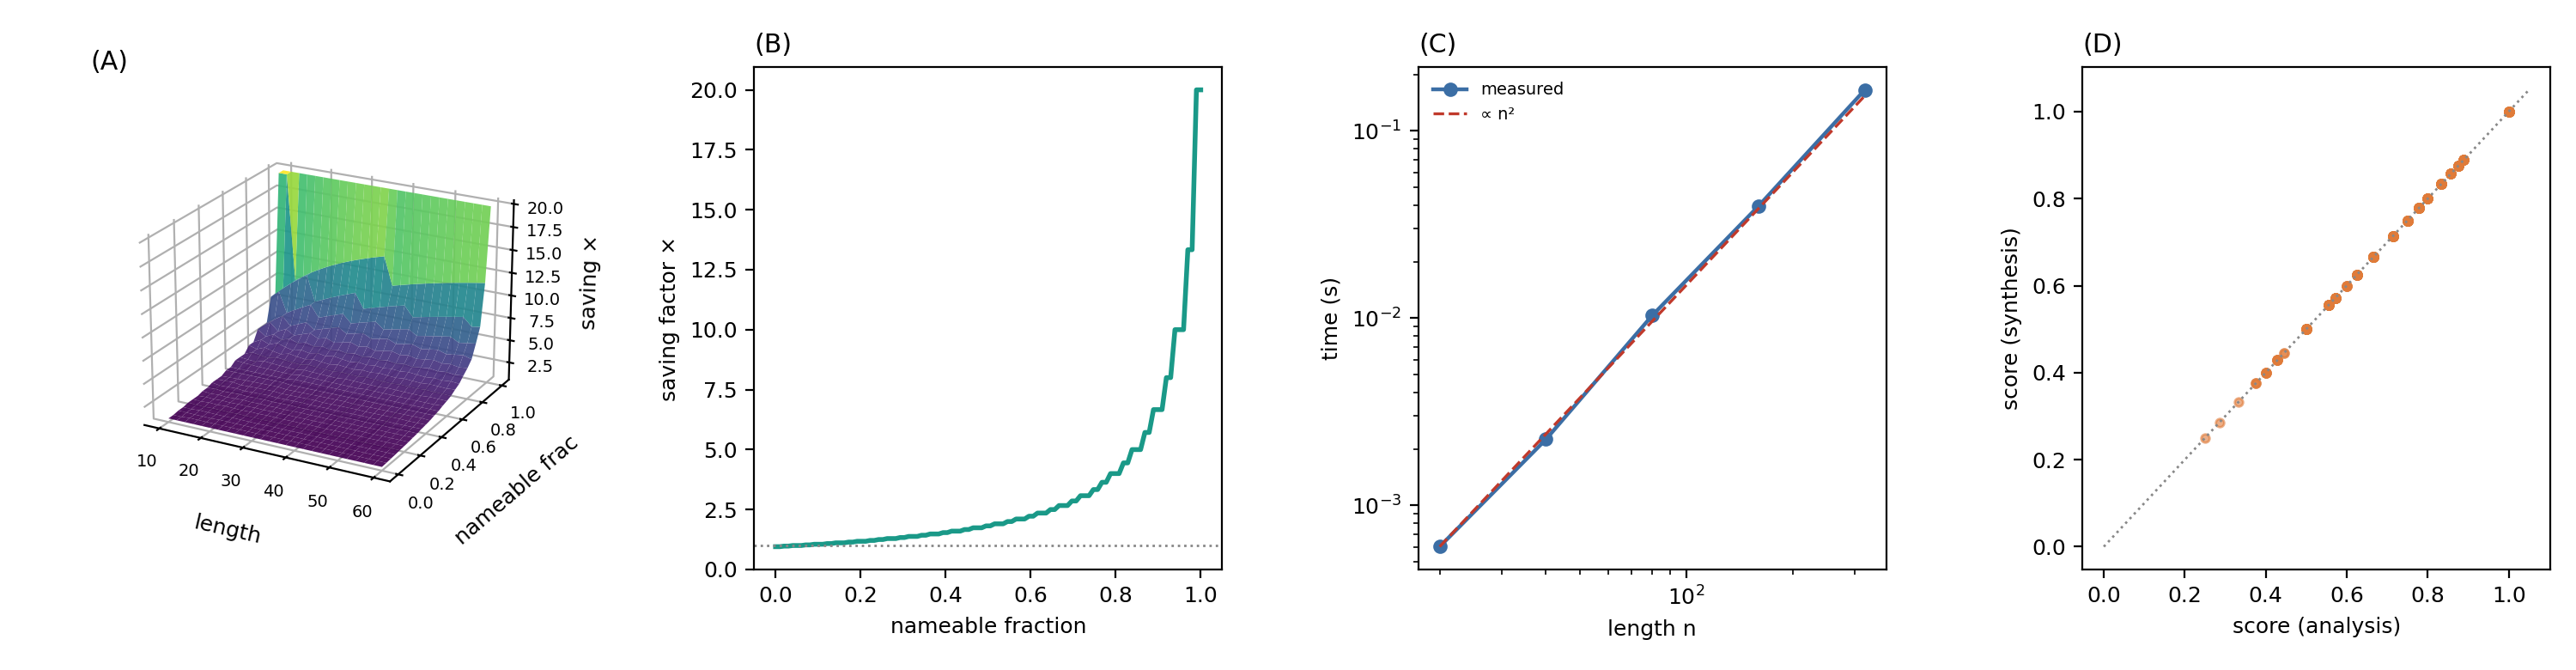
\includegraphics[width=\textwidth]{figures/panel_4_duality.png}
\caption{\textbf{Duality and the contingent saving} (\Cref{sec:duality,%
sec:algorithm}). (A) The saving factor
$1/((c_{\mathrm{sym}}/c_{\mathrm{ac}})+(1-\phi))$ over (stream length, nameable
fraction $\phi$): it rises with $\phi$ and is \emph{independent of length},
exactly as \Cref{cor:cheaper} predicts. (B) At fixed length the saving curve runs
from $1\times$ (no saving) at $\phi=0$ up toward the $c_{\mathrm{ac}}/
c_{\mathrm{sym}}=20\times$ ceiling at $\phi=1$; the measured mean over random
streams is $3.1\times$. (C) The alignment dynamic program's measured runtime
tracks the $\propto n^2$ guide (empirical doubling ratios $3.7$--$4.4$ against the
predicted $4.0$), confirming $\bigOh(nN)$ (\Cref{thm:complexity}). (D) The
analysis and synthesis scores coincide on the diagonal in $300/300$ trials---the
one dynamic program computes both directions (\Cref{thm:duality}).}
\label{fig:duality}
\end{figure*}

\begin{proof}
The saving factor is the quotient of the two costs, and rearranging
$n\,c_{\mathrm{sym}}+r\,c_{\mathrm{ac}}=n\,c_{\mathrm{ac}}\bigl((c_{\mathrm{sym}}/
c_{\mathrm{ac}})+(1-\phi)\bigr)$ gives the stated form. It exceeds $1$ exactly
when $(c_{\mathrm{sym}}/c_{\mathrm{ac}})+(1-\phi)<1$, i.e.\ when
$\phi>c_{\mathrm{sym}}/c_{\mathrm{ac}}$. As $\phi\to1$ the denominator
$\to c_{\mathrm{sym}}/c_{\mathrm{ac}}$ and the factor $\to c_{\mathrm{ac}}/
c_{\mathrm{sym}}$; as $\phi\to0$ (so $r\to n$) the denominator $\to
1+c_{\mathrm{sym}}/c_{\mathrm{ac}}\to1$ and the factor $\to1$. The whole-item
search never costs \emph{more} than per-track (the denominator adds only the
small $c_{\mathrm{sym}}/c_{\mathrm{ac}}$ overhead), but its advantage vanishes
continuously as the nameable fraction falls, so the saving is contingent on
$\phi$ and bounded by the cost ratio.
\end{proof}

\begin{remark}[The saving is measured, not promised]
\label{rem:phi-empirical}
Because the saving factor is exactly $1/\bigl((c_{\mathrm{sym}}/c_{\mathrm{ac}})+
(1-\phi)\bigr)$, its value on any corpus is fixed by the nameable fraction
$\phi$ that corpus and recogniser actually achieve---never by the calculus. The
validation (\Cref{sec:validation}) measures this directly: over randomly drawn
streams the \emph{mean} saving is a modest $3.1\times$ (not the $c_{\mathrm{ac}}/
c_{\mathrm{sym}}=20\times$ ceiling), with instances near $\phi=0.065$ that save
essentially nothing---precisely the worst-case regime this corollary now names
rather than hides.
\end{remark}

\begin{remark}[Where the savings come from]
\label{rem:savings}
The economy is a direct dividend of the two structural results: the sequence
narrows each constituent's ambiguity set so a cheap name suffices
(\Cref{prop:context}), and the floor principle forbids paying for resolution past
sufficiency (\Cref{thm:sufficiency}). The expensive acoustic stage runs on the
residual only---exactly the unnamed and name-colliding constituents
(\Cref{prop:residual})---so cost scales with how much of the stream is genuinely
unidentifiable, not with its length.
\end{remark}

% ============================================================================
\section{Worked example}
\label{sec:example}
% ============================================================================

We illustrate the pipeline on a small synthetic instance to make the objects
concrete.

\begin{example}[Two mixes, shared content, different sequence]
\label{ex:two-mixes}
Let the public pool contain tracks with name-handles
$\{A,B,C,D,E\}$. Two recorded mixes draw on the same five tracks:
\[
\text{Mix }1:\ \sig_1=(A,B,C,D,E),\qquad
\text{Mix }2:\ \sig_2=(A,C,B,E,D).
\]
Their content sets are identical, $\{\!\{A,B,C,D,E\}\!\}$, so a bag-of-tracks
search cannot distinguish them (\Cref{thm:signature}(ii)). Their signatures
differ: aligning $\sig_1$ to $\sig_2$ with $\mu=\delta=1$ requires moving $B,C$
and $D,E$, giving a positive alignment cost, so the two are separated as distinct
items. Now suppose a listener captures a low-fidelity recording of Mix~1 in which
$C$ is unnamed (an unreleased ID) and $D$ is misheard as a same-titled but
acoustically distinct edit $D'$. Acquisition (\Cref{alg:acquire}) yields
$\sig=(A,B,\bot,D',E)$; the residual is positions $3$ (gap) and $4$
(substitution). Matching (\Cref{alg:match}) against the library aligns $\sig$ to
$\sig_1$ at cost $\delta+\mu=2$, normalised
$\algn=2/(\delta\cdot 5)=0.4$. If $\eps\ge 0.4$ the match is admissible
(\Cref{thm:admissibility}): Mix~1 is correctly identified despite two of five
constituents being wrong, and the residual $\{3,4\}$ is exactly where an acoustic
pass is owed (\Cref{prop:residual})---position $3$ to name the ID, position $4$
to separate $D$ from $D'$. No acoustic work is done on $A,B,E$, which their names
already placed.
\end{example}

This single example exercises every result: content non-identity
(\Cref{thm:signature}), least-sufficient handles with acoustic descent only on
the residual (\Cref{cor:name-first,prop:residual}), and convergence-only
admissibility absorbing local errors (\Cref{thm:admissibility}).

\begin{figure*}[!htbp]
\centering
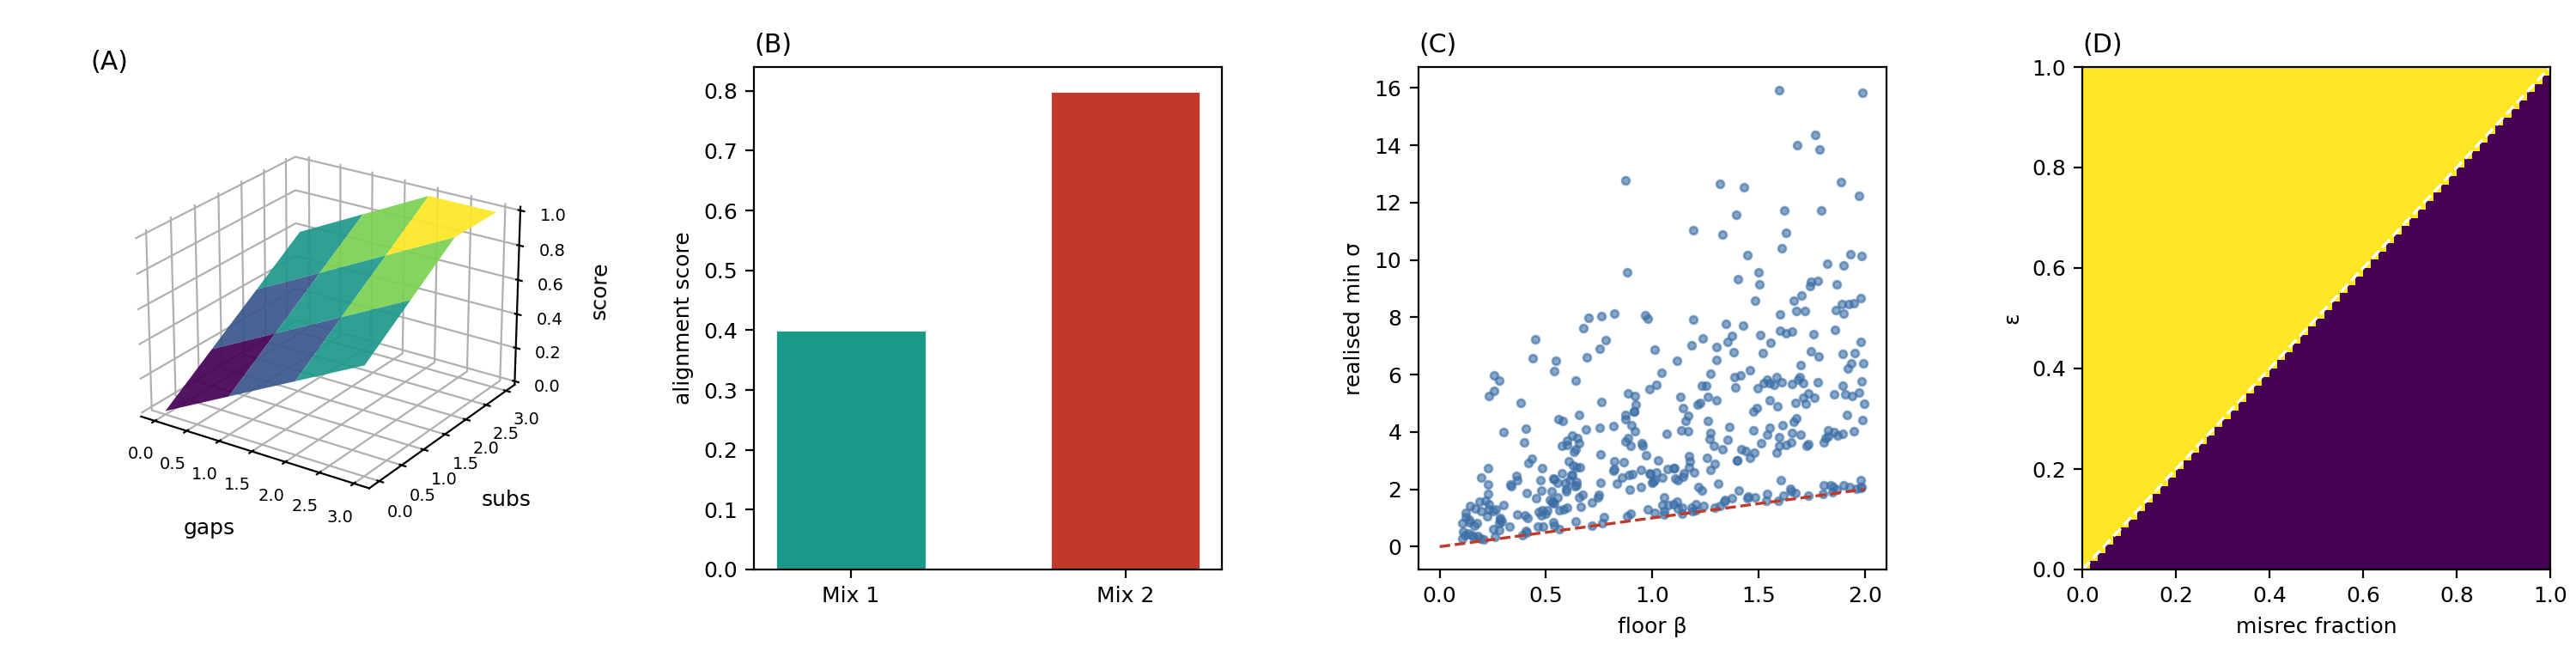
\includegraphics[width=\textwidth]{figures/panel_5_worked_example.png}
\caption{\textbf{End-to-end behaviour on \Cref{ex:two-mixes}}. (A) The alignment
score of a degraded capture of Mix~1 to Mix~1, as a function of injected gaps and
substitutions: the surface rises smoothly, so partial degradation stays
admissible. (B) The degraded capture $\sig=(A,B,\bot,D',E)$ scores $0.4$ to
Mix~1 and $0.8$ to Mix~2---correctly identified despite two of five constituents
wrong. (C) The realised minimum $\str$ tracks the floor $\flo$ across $400$
random graphs, all on or above the line. (D) The admissibility phase map
$\{\text{misrec}\le\eps\}$, the operating region of \Cref{thm:admissibility}.}
\label{fig:worked}
\end{figure*}

% ============================================================================

% ============================================================================
\section{Evaluation protocol}
\label{sec:evaluation}
% ============================================================================

The theory is structural and its guarantees are proved; empirical evaluation
concerns how well concrete recognisers and cost settings realise the framework on
real streams. We specify a reproducible protocol rather than report numbers, so
that an implementation can be measured against it.

\subsection{Datasets}

\begin{enumerate}[leftmargin=1.4em,itemsep=2pt]
\item \textbf{Reference streams with ground-truth tracklists.} Recorded mixes,
radio shows, or sets for which an authoritative ordered tracklist (with onset
times) is known---from published cue sheets or annotated corpora
\citep{schwarz2018dj,sonnleitner2016landmark}. Each supplies a ground-truth
signature $\sig^{\ast}$.
\item \textbf{Degraded captures.} For each reference stream, generate captures
with controlled degradations: additive noise, transcoding, partial occlusion,
segmentation perturbation, and a controlled fraction of constituents forced
unlabelled or name-collided. These test convergence-only admissibility
(\Cref{thm:admissibility}) against a known misrecognition fraction.
\item \textbf{Shared-content distractors.} Pairs of distinct items with high
content-set overlap but different sequences, to test that the signature
distinguishes items a content search conflates (\Cref{thm:signature}(ii)).
\end{enumerate}

\subsection{Metrics}

\begin{enumerate}[leftmargin=1.4em,itemsep=2pt]
\item \textbf{Item retrieval.} Precision, recall, and mean reciprocal rank for
returning the correct library item given a (possibly degraded) query stream---the
whole-item analogue of track identification.
\item \textbf{Sequence accuracy.} Alignment score $\algn(\sig,\sig^{\ast})$
between recovered and ground-truth signatures, and the fraction of positions in
the accounted match (\Cref{def:accounted}); reported against the injected
misrecognition fraction to trace the tolerance curve of \Cref{cor:partial}.
\item \textbf{Content--sequence separation.} On the shared-content distractor
pairs, the rate at which the system correctly separates items with identical
content sets, contrasted with a content-set baseline (which by construction
cannot, \Cref{thm:signature}(ii)).
\item \textbf{Resolution economy.} The residual fraction $r/n$ and the acoustic
invocation count, versus a per-constituent-fingerprint baseline, to measure the
saving of \Cref{cor:cheaper}.
\item \textbf{Decline calibration.} On queries with no true library match, the
rate of correct \textsc{decline} versus forced false matches.
\end{enumerate}

\subsection{Ablations}

\begin{enumerate}[leftmargin=1.4em,itemsep=2pt]
\item \textbf{Name-only vs name+acoustic.} Disabling the acoustic descent
isolates the value of resolving the residual (\Cref{prop:residual}).
\item \textbf{Tolerance $\eps$.} Sweeping $\eps$ traces the admissibility
boundary of \Cref{thm:admissibility} and locates the operating point balancing
missed matches against false accepts.
\item \textbf{Candidate threshold $\theta$.} Sweeping $\theta$ trades matching
speed (\Cref{thm:complexity}(iii)) against recall.
\item \textbf{Global vs local alignment.} Comparing modes
(\Cref{rem:local}) on ``is this the item'' versus ``does this contain the item''
queries.
\end{enumerate}

\begin{remark}[What the protocol tests, and what it cannot]
\label{rem:eval-scope}
This protocol is distinct from the numerical validation of \Cref{sec:validation}.
The validation instance-checks the theorems by exact computation on synthetic
graphs and signatures---confirming they hold where they must and quantifying the
one contingent constant (the nameable fraction). This evaluation protocol instead
measures the realisation of the framework by \emph{concrete} recognisers on
\emph{real} streams; it does not test the theorems, which are proved. The proved
guarantees---floor positivity, signature invariance, convergence-only
admissibility, duality---hold for any recogniser and any cost setting satisfying
the stated assumptions; the protocol measures how favourable the constants are on
real data (nameable fraction, residual size, tolerance headroom), which is an
empirical property of the recognisers and streams, not of the calculus.
\end{remark}

% ============================================================================
\section{Discussion}
\label{sec:discussion}
% ============================================================================

\subsection{What the paper establishes}

The paper reframes audio search for continuous items around three proved facts.
The identity of a continuous item is its \emph{sequence} of constituents, not its
content set, because content is drawn from a shared public pool while order is
essentially unique to the producing item (\Cref{thm:signature}). Constituent
recognition against an open pool is \emph{floored}---no exact identification
exists---so each constituent should be resolved only to its \emph{least
sufficient identifier}, typically a name, with expensive acoustic resolution
reserved for the residual it cannot place (\Cref{thm:floor,thm:sufficiency,%
cor:name-first}). And matching is \emph{convergence-only} sequence alignment, so
partial and noisy recognition still identifies the whole item provided the
sequence globally aligns (\Cref{thm:admissibility}). Analysis and synthesis are
the same alignment in two directions (\Cref{thm:duality}), so one engine both
recognises and generates.

\subsection{Honest limitations}

We mark the load-bearing assumptions. First, \emph{segmentation} is taken as
given: the theory is stated over a constituent sequence, and errors in finding
constituent boundaries appear to the matcher as insertions/deletions, absorbed by
convergence-only admissibility up to the tolerance $\eps$ but not beyond; a poor
segmenter degrades the constants. Second, \emph{non-completability}
(\Cref{def:noncompletable}) is an order condition we assume of the pool; it is
what forces the floor, and a genuinely closed, fully enumerated catalogue would
not satisfy it (in which case exact identification could exist and the
least-sufficient economy would still hold as an efficiency but not as a
necessity). Third, the \emph{alignment cost model} (\Cref{def:alignment}) uses
uniform substitution and gap costs; handle-dependent costs (a substitution
between acoustically close handles cheaper than between distant ones) are a
natural refinement the framework accommodates but that requires a concrete handle
metric. Fourth, the \emph{ambiguity set} narrowing (\Cref{prop:context}) assumes
a context model that predicts plausible successors; its quality determines how
small $A(v)$, hence how cheap the least sufficient identifier, actually is, and it
does nothing at all for the first constituent, which has no resolved left context
and faces the full pool (validated in \Cref{fig:signature}(C): mean $\abs{A}=69$
at context length $0$). Fifth, and consequently, the \emph{complexity saving} is
contingent, not structural: \Cref{cor:cheaper} shows the whole-item search beats
per-track fingerprinting only by the nameable fraction $\phi$, degrading to no
saving as $\phi\to0$ (measured mean $3.1\times$, \Cref{fig:duality}); the
opening-track cost persists regardless of stream length.

\subsection{Relation to single-track search}

The framework contains single-track search as a degenerate case: an item of
length $n=1$ has signature a single handle, and matching reduces to handle
lookup---ordinary track identification. The contribution is the $n>1$ regime,
where the sequence carries the identity and the per-constituent economy applies.
Conversely, a single-track recogniser is a natural provider for the
$\textsc{Name}$ and $\textsc{Acoustic}$ stages: the paper builds \emph{on top of}
track recognition rather than replacing it, adding the sequence-identity and
whole-item search layer that track recognition does not model.

% ============================================================================
\section{Conclusion}
\label{sec:conclusion}
% ============================================================================

Most listening is to continuous items---radio, mixes, sets, parties---not to
isolated tracks, yet audio search has been built for the isolated track. We have
given an algorithm that searches a continuous item as a single object. Its
foundation is that the identity of such an item is the \emph{sequence} in which
it arranges its constituents, not the constituents themselves, which are drawn
from a shared public pool and cannot individuate the item. Because recognising a
constituent against an open pool is floored, one resolves each constituent only
to the least sufficient handle that places it in the sequence---usually its
name---and pays the cost of acoustic analysis only on the residual of unnamed or
name-colliding constituents. Matching is sequence alignment with
convergence-only admissibility, so a whole item is identified from a partial,
noisy recognition provided its sequence globally aligns, and the search returns
an accounted match together with an honest residual of what it could not place.
Recognising an item and generating one in its manner are the same alignment read
in opposite directions. The outcome is a music search at the granularity of the
listening experience: one searches for the set, the show, the party---the whole
item---rather than for every song inside it, and does so more cheaply than
recognising each song, because the sequence itself supplies most of the
individuation that a per-track fingerprint would have to compute.

% ============================================================================
\bibliographystyle{plainnat}
\bibliography{references}
% ============================================================================

\end{document}

